\documentclass[11pt]{article}

%%% Load some useful packages:
%% "New" LaTeX2e graphics support.
\usepackage{graphicx}
%%	using final option to force graphics to be included even in draft mode
%\usepackage[final]{graphicx}

%% Make subsubsections numbered and included in ToC
\setcounter{secnumdepth}{3}
\setcounter{tocdepth}{3}

%% Package to linebreak URLs in a sane manner.
\usepackage{url}

%% Define a new 'smallurl' style for the package that will use a smaller font.
\makeatletter
\def\url@smallurlstyle{%
  \@ifundefined{selectfont}{\def\UrlFont{\sf}}{\def\UrlFont{\small\ttfamily}}}
\makeatother
%% Now actually use the newly defined style.
\urlstyle{smallurl}

%% Make margins less ridiculous
\usepackage{fullpage}

%% Allows insertion of fixme notes for future work
\usepackage[footnote, nomargin]{fixme}

%%%% Turned off for tech report, should be turned on for research portfolio
%% Turn on double spacing
%\usepackage{setspace}
%\doublespacing

%% Make URLs clickable
\usepackage[colorlinks, bookmarks=true]{hyperref}
\usepackage[all]{hypcap}


%% Since I'm using the LaTeX Makefile that uses dvips, I need this
%% package to make URLs break nicely
\usepackage{breakurl}

\usepackage{array}

%% Make table cross pages.
\usepackage{longtable}

\begin{document}

\title{Results from the 2008 Classroom Evaluation of Hackystat}

\author{Shaoxuan Zhang \\
				 Philip M. Johnson \\
\em  Collaborative Software Development Laboratory \\
\em  Department of Information and Computer Sciences \\
\em  University of Hawai'i \\
\em  Honolulu, HI 96822 \\
\em  sz@hawaii.edu \\
}

\date{\today}
\maketitle

%%\tableofcontents

\graphicspath{{figures/}} 
\DeclareGraphicsExtensions{.eps} 

\begin{abstract}
This report presents the results from a classroom evaluation of Hackystat by ICS 413 students at the end of Fall, 2008.  The students had used Hackystat v8 for approximately four weeks at the time of the evaluation.  The survey requests their feedback regarding the installation, configuration, overhead of use, usability, utility, and future use of the Hackystat (Version 8)\footnote{All future references to ``Hackystat'' implies Version 8; other versions of Hackystat will be referred explicit such as Version 7 and Version 6}. This classroom evaluation is a semi-replication of the evaluations performed on Hackystat in Fall 2003\cite{csdl2-03-13} and Fall 2006\cite{csdl2-07-02}. As Hackystat has changed significantly since Hackystat Version 7 in 2006, some of the evaluation questions were changed. 

The data from this evaluation, in combination with the data from the 2003 and 2006 evaluations, provides an interesting perspective on the past, present, and possible future of Hackystat. Hackystat is an completely rebuilt version, which is organized as a collection of loosely coupled software services such as SensorBase, DailyProjectData and Telemetry, which together provide better extensibility and flexibility compared to the old versions. The result shows that, though there are some regressions on installation and overhead of use, Hackystat did successfully accomplish its utility to facilitating development. 
\end{abstract}

\section{Methodology}
At the end of the Fall 2008 semester, the students in ICS 413 were contacted by email and asked to respond to the following questionnaire soliciting their opinions regarding Hackystat. The graduate student researcher on this project (Shaoxuan Zhang, sz@hawaii.edu) provided each of the students a ``secret'' code. The correspondences between the secret codes and the students are only known by the graduate student, but not the instructor of the class, in order to avoid the potential for bias to ``please'' the instructor/designer who would presumably be gratified by positive responses to the questionnaire. Response was optional, but the students were offered extra credit points for providing their opinions. The list of names who should be awarded extra credit was sent to the class instructor without identifying individual responses. The students were asked to reply within a week. Eighteen out of the nineteen students contacted provided responses. 

In addition, we log students' usage of the system, which is not awared by students, and we compare the logging data with the feedbacks from the survey.

The complete questionnaire follows:

\begin{quote}
\sl
{\bf \em Hackystat Evaluation}

Hackystat is a long term research project concerned with improving the effectiveness and efficiency of software engineering metrics collection and analysis.  Since 2003, we have periodically conducted a survey of students in ICS software engineering classes to assess the current strengths and weaknesses of the system.

To preserve anonymity,  while also ensuring that only ICS students respond and respond only once, we ask you to provide the "secret code" that you randomly selected in class.   To enable credit for completing this evaluation, only the graduate student researcher on this project (Shaoxuan Zhang) will know which code corresponds to you.  He will provide a list of names who should be awarded credit to the class instructor without identifying individual responses.  You can also contact Shaoxuan if you want your data deleted from analysis after you've submitted it.

If you want to go back and change your responses, simply fill out the entire form again.  We will discard all but the most recently submitted entry for a given code.

This survey contains 17 questions and we expect that you will need about 10 minutes to complete it.

Thank you very much for your help!  We take your views very seriously: prior responses to this survey have led to far-reaching changes in Hackystat.

Before filling out this questionnaire, you might want to take a look at the following image for the Software ICU to refresh your memory:

\url{http://csdl.ics.hawaii.edu/~johnson/portfolio.gif}

* Required
\begin{enumerate}

\item Installing the Eclipse IDE sensor was: *
\begin{itemize}
\item Very Easy
\item Easy
\item Neither easy nor difficult
\item Difficult
\item Very Difficult
\end{itemize}

\item Installing the Ant sensors (JUnit, SCLC, Emma, etc.) was: *
\begin{itemize}
\item Very Easy
\item Easy
\item Neither easy nor difficult
\item Difficult
\item Very Difficult
\end{itemize}

\item Please provide any feedback you can on the problems you experienced during sensor installation and server configuration, as well as any suggestions you have to make this easier in future.

\item The amount of overhead required to collect Hackystat data (after successful installation and configuration of sensors) was: *
\begin{itemize}
\item Very Low
\item Low
\item Neither low nor high
\item High
\item Very High
\end{itemize}

\item The amount of overhead required to run Hackystat analyses was: *
\begin{itemize}
\item Very Low
\item Low
\item Neither low nor high
\item High
\item Very High
\end{itemize}

\item Please provide any feedback you can on Hackystat overhead, as well as any suggestions you have to reduce the overhead in future.

\item Did you encounter any problems while collecting data? Was there any kind of data that you failed to collect? If yes, please explain.

\item How did you feel about sharing your software development data with other members of the class? *

\item How frequently did you use the telemetry page? *
\begin{itemize}
\item Every day or more
\item 2-3 times a week
\item Once a week
\item Less than once a week
\item Never
\end{itemize}

\item If you used the Telemetry page, what were you trying to find out?

\item How frequently did you use the Software ICU? *
\begin{itemize}
\item Every day or more
\item 2-3 times a week
\item Once a week
\item Less than once a week
\item Never
\end{itemize}

\item If you used the Software ICU, please check the vital signs that were useful to you. *
\begin{itemize}
\item Coverage
\item Complexity
\item Coupling
\item Churn
\item Size
\item DevTime
\item Commit
\item Build
\item Test
\item None of the above
\end{itemize}

\item Did you feel the Software ICU colors accurately reflected the "health" of your project? If not, why not? *

\item Were you able to use the Software ICU to improve your software's quality and/or your team's process? If so, in what ways? If not, why not? *

\item Please provide any other feedback you would like regarding Telemetry and the Software ICU, as well as any suggestions you have on how we can improve the system.

\item If I was a professional software developer, using Hackystat at my job would be: *
\begin{itemize}
\item Very feasible
\item Somewhat feasible
\item Neither feasible nor infeasible
\item Somewhat infeasible
\item Very infeasible
\end{itemize}

\item Please provide any other feedback you can on the feasibility of Hackystat in a professional setting, as well as any suggestions you have on how its feasibility could be improved. 

\end{enumerate}

\end{quote}


\section{Results form Questionnaire}
This section presents the responses from the respondents to each of the questions. For the "short answer" questions, I corrected misspellings and minor grammatical errors to improve readability.  

\begin{center}
\footnotesize
\begin{longtable}{|m{0.4\textwidth}|m{0.6\textwidth}|}
\hline 
{\bf Question}&{\bf Response}\endhead \hline
1. Installing the Eclipse IDE sensor was:
\label{q1}
\begin{itemize}
\item Very Easy
\item Easy
\item Neither easy nor difficult
\item Difficult
\item Very Difficult
\end{itemize}
&
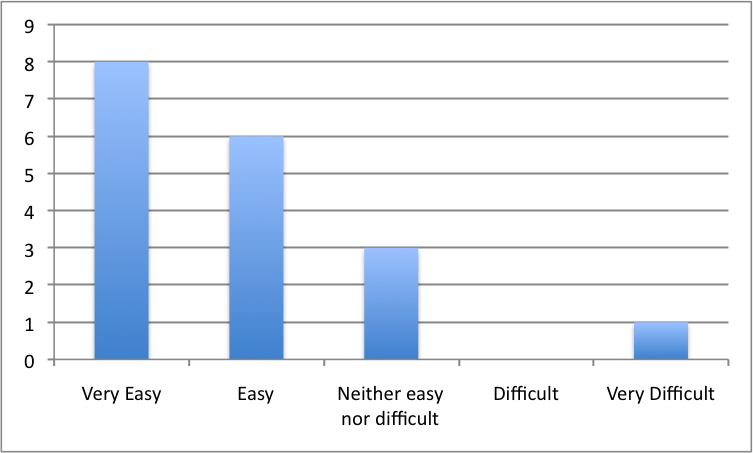
\includegraphics[width=0.6\textwidth]{Q01-InstallEclipseSensor} \\ \hline

2. Installing the Ant sensors (JUnit, SCLC, Emma, etc.) was:
\begin{itemize}
\item Very Easy
\item Easy
\item Neither easy nor difficult
\item Difficult
\item Very Difficult
\end{itemize}
&
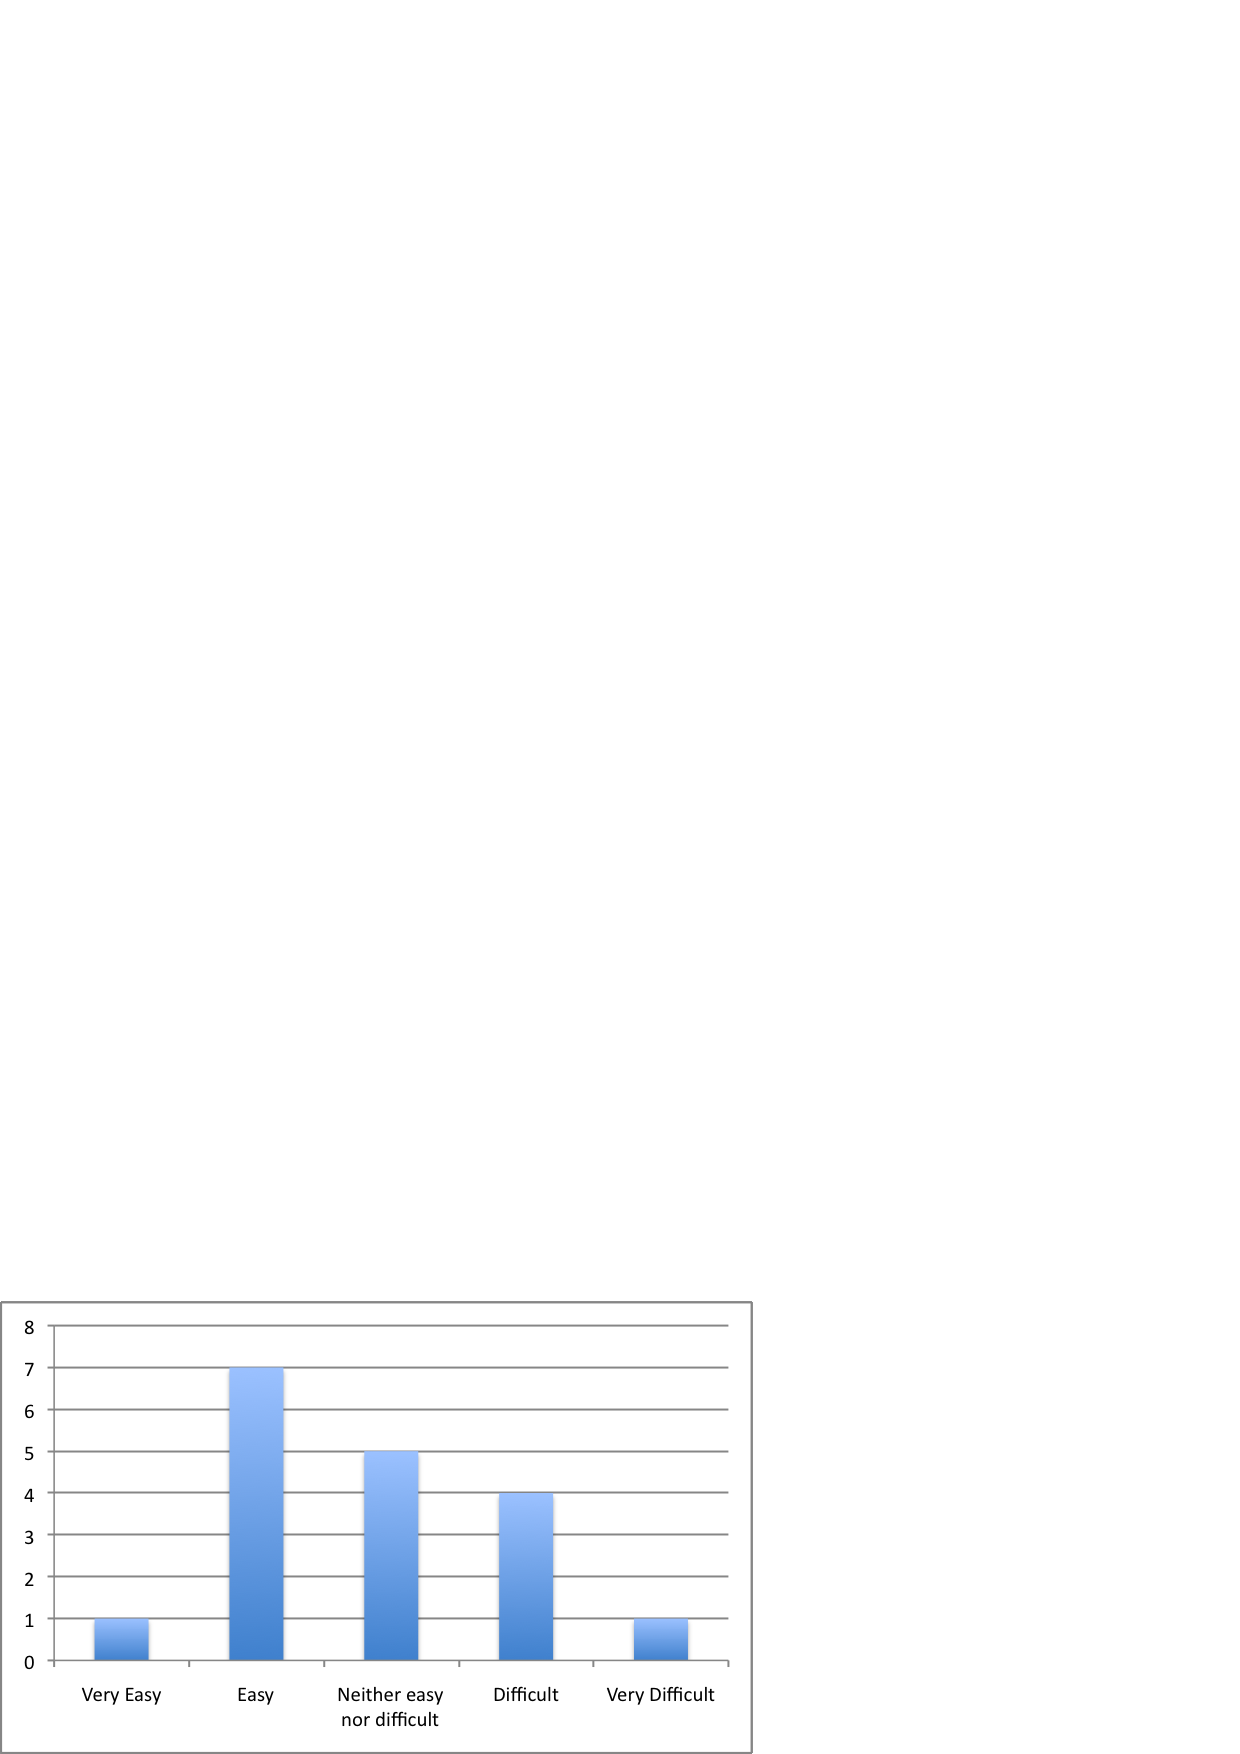
\includegraphics[width=0.6\textwidth]{Q02-InstallAntSensor} \\ \hline

\end{longtable}
\end{center}


3. Please provide any feedback you can on the problems you 
experienced during sensor installation and server con�guration, as well as any suggestions you have to make this easier 
in future.
\begin{itemize}
\item I could not figure out what step makes a .hackystat directory. My .hackystat directory automatically generated in my Documents and Settings directory which has a blank space in directory name. I am still not sure how to move this folder to other. The instalation of all sensors was pretty well described at the project homepage and there was no problems I have met during the installation. 

\item Both the installation and sending sensor data was easy.  However, tracking down whenever there is a problem with the sensor is not so easy.  A troubleshooting page in the near future?

\item Installing the sensors was pretty straightforward.  I didn't have any problems.

\item Case sensitivity was one problem between user and Hackystat, but it was fixed.  

If it is possible to have a .EXE that will automatically create environment variables and also install files into a local directory will be awesome.

\item I did have one small hang up when installing the Ant sensors: If I remember correctly I was getting a noclassdefinition error whenever a sensor ran. I was running java 1.5. I fixed it by downloading the jaxb libraries since the errors were referring to that. It could be not related to jaxb at all, but it worked after that. Otherwise, I had no problems whatsoever installing the sensors.

\item Everything went smooth with the instructions given and the verification after each step.

\item Personally I didn't run into any problems but some of the other students did. The sensors aren't difficult to install per se, but there are a lot of steps involved and it's easy to get lost while installing them. Maybe an automated installer can be created that searches for the Ant tools (maybe the user can provide a search directory) and will configure and install the sensors for the user.

\item What made it hard was that all the instructions were not in one page.  I had to go from one page to another and then to another.  There should be instructions from STEP 1 to the end and provide proper links to the step by step process.

\item First of all, the manual is too long. I do like your goal to analyze the software project, but if it wasn't required by this class, maybe I wouldn't think I want to use it, because it looks too complicated. 

Also there are too many things that we need to download and install. If you want to encourage people to use this more, maybe you should provide a package of all the tools somehow. 

For example, before it took a long time to install Apache, MySQL, PHP, and Perl, but now somebody offers a package called XAMPP, which is a combination of all of those, and entire installation finishes in 3 minutes. Something like that should be given. 

\item There is a lot of documentation in a lot of different places.  It was confusing trying to figure out what to read in what order, and whether or not it was relevant to me.

\item Some the installation instructions could benefit from "write once, use many times" as they're repeated, which causes some people to start glossing over the instructions and then there's a couple that are slightly different and people (like me) won't notice the difference.

\item The walkthrough was great, which made the installation easy.

\item The only problem I had was the installation of the ant sensor. I mean configuring it on Eclipse was easy especially when I try to run Emma, JUnit, FindBugs and all that from Eclipse it is sending stuff to Hackystat but when I checked my software ICU I didn't have any data on Build (all it says was N/A). And little did I know that when you run the ant sensors on Eclipse it only registers all the data to Hackystat JUnit, Emma, Checkstyle and such except BUILD. And I was told  that running the BUILD on the command line works but not on Eclipse. So I tried that and YES that works. So is there a way to make it work on Eclipse when you run all the ant sensors and it sends all the data to Hackystat including the BUILD data?

\item When we ran the svn sensor, the build would fail if there are any commits from members not identified in our local Usermap.xml.  Instead of looking for all commit records from all users within 24 hours, perhaps it could filter out and only look for records inside our UserMap.xml.

\item The installation documentation must be read carefully.  It may be easier to create a hackystat.build.xml with all the build targets, then import that file into each *.build.xml and call the sensor from the tasks.

\item The most challenging sensor to get up and running was the SVN sensor.  Other than that, the others seemed fairly easy to install.

\end{itemize}

\begin{center}
\footnotesize
\begin{longtable}{|m{0.4\textwidth}|m{0.6\textwidth}|}
\hline 
{\bf Question}&{\bf Response}\endhead \hline
4. The amount of overhead required to collect Hackystat data (after successful installation and configuration of sensors) was: *
\begin{itemize}
\item Very Low
\item Low
\item Neither low nor high
\item High
\item Very High
\end{itemize}
&
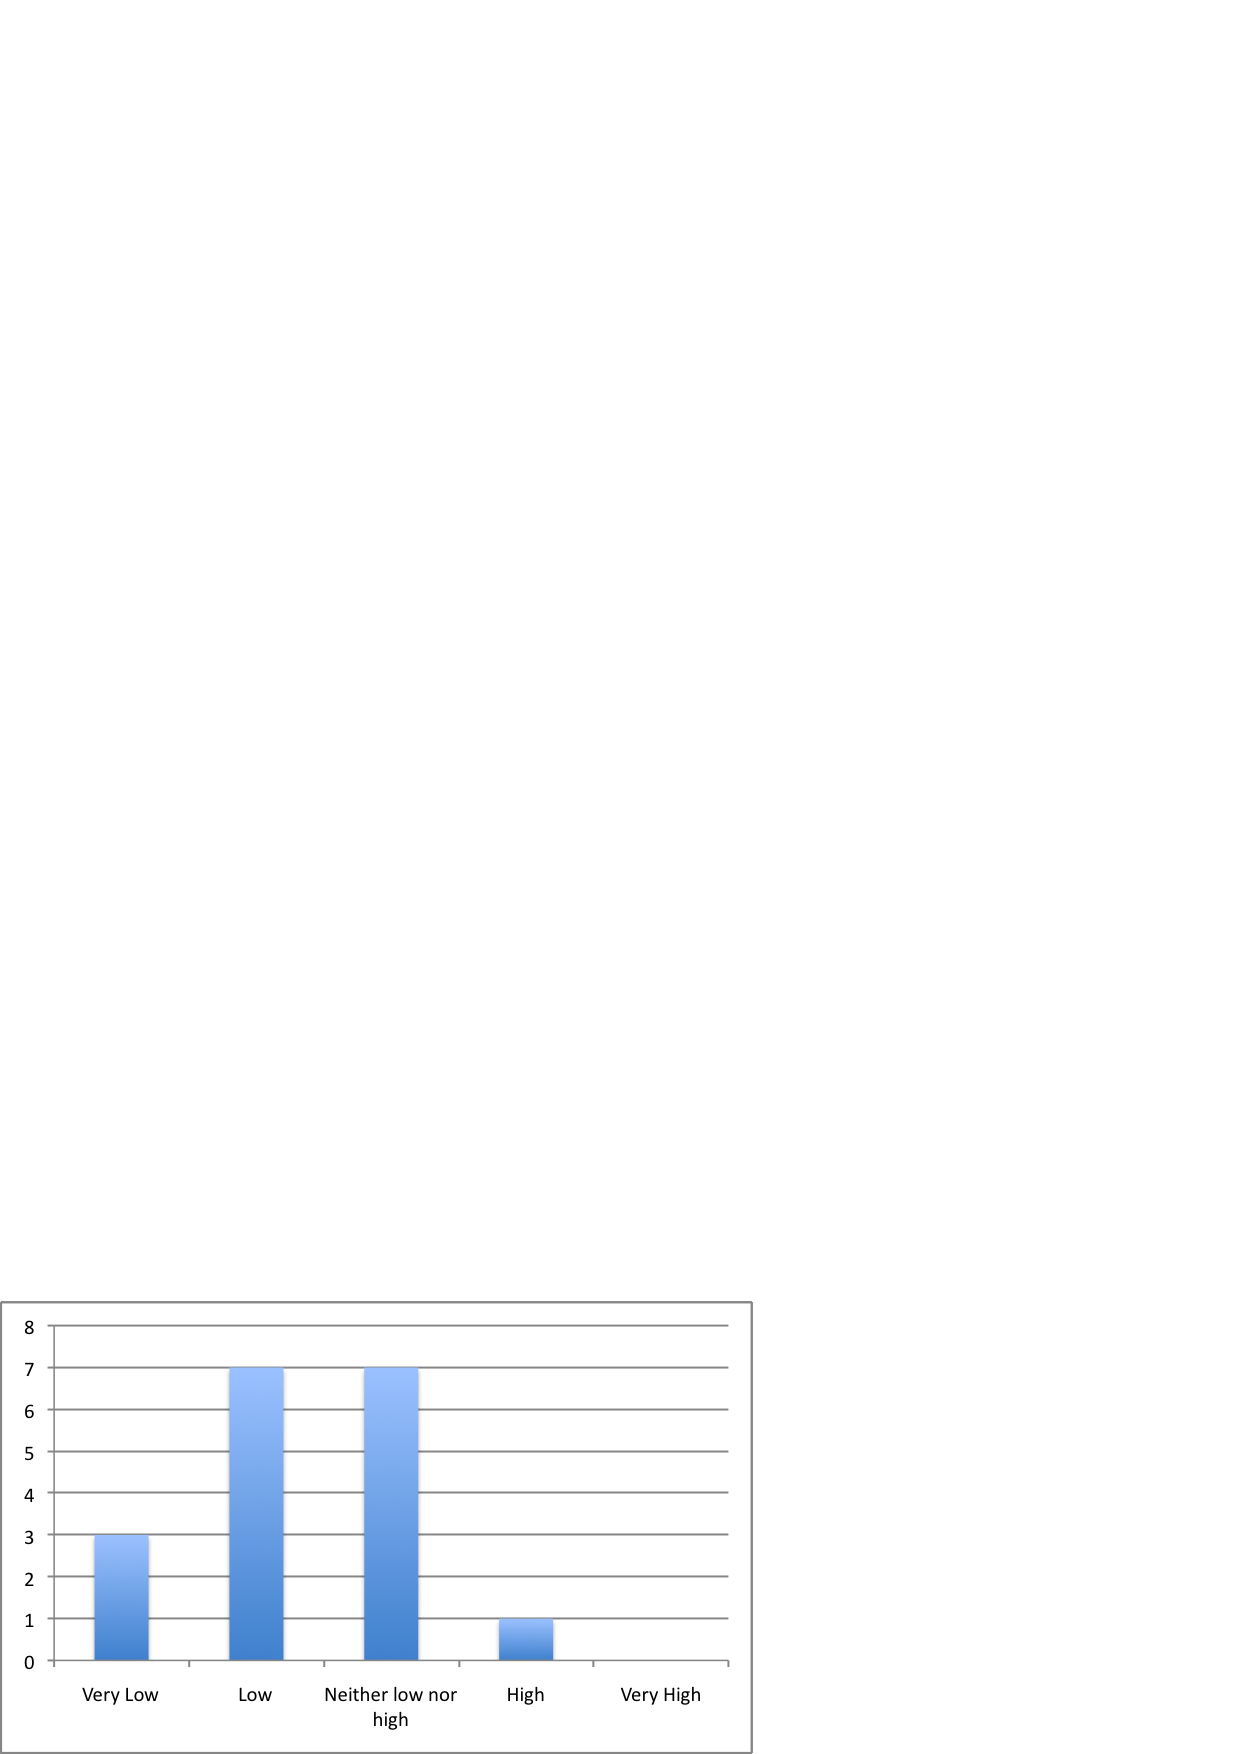
\includegraphics[width=0.6\textwidth]{Q04-DataCollectOverhead} \\ \hline

5. The amount of overhead required to run Hackystat analyses was: *
\begin{itemize}
\item Very Low
\item Low
\item Neither low nor high
\item High
\item Very High
\end{itemize}
&
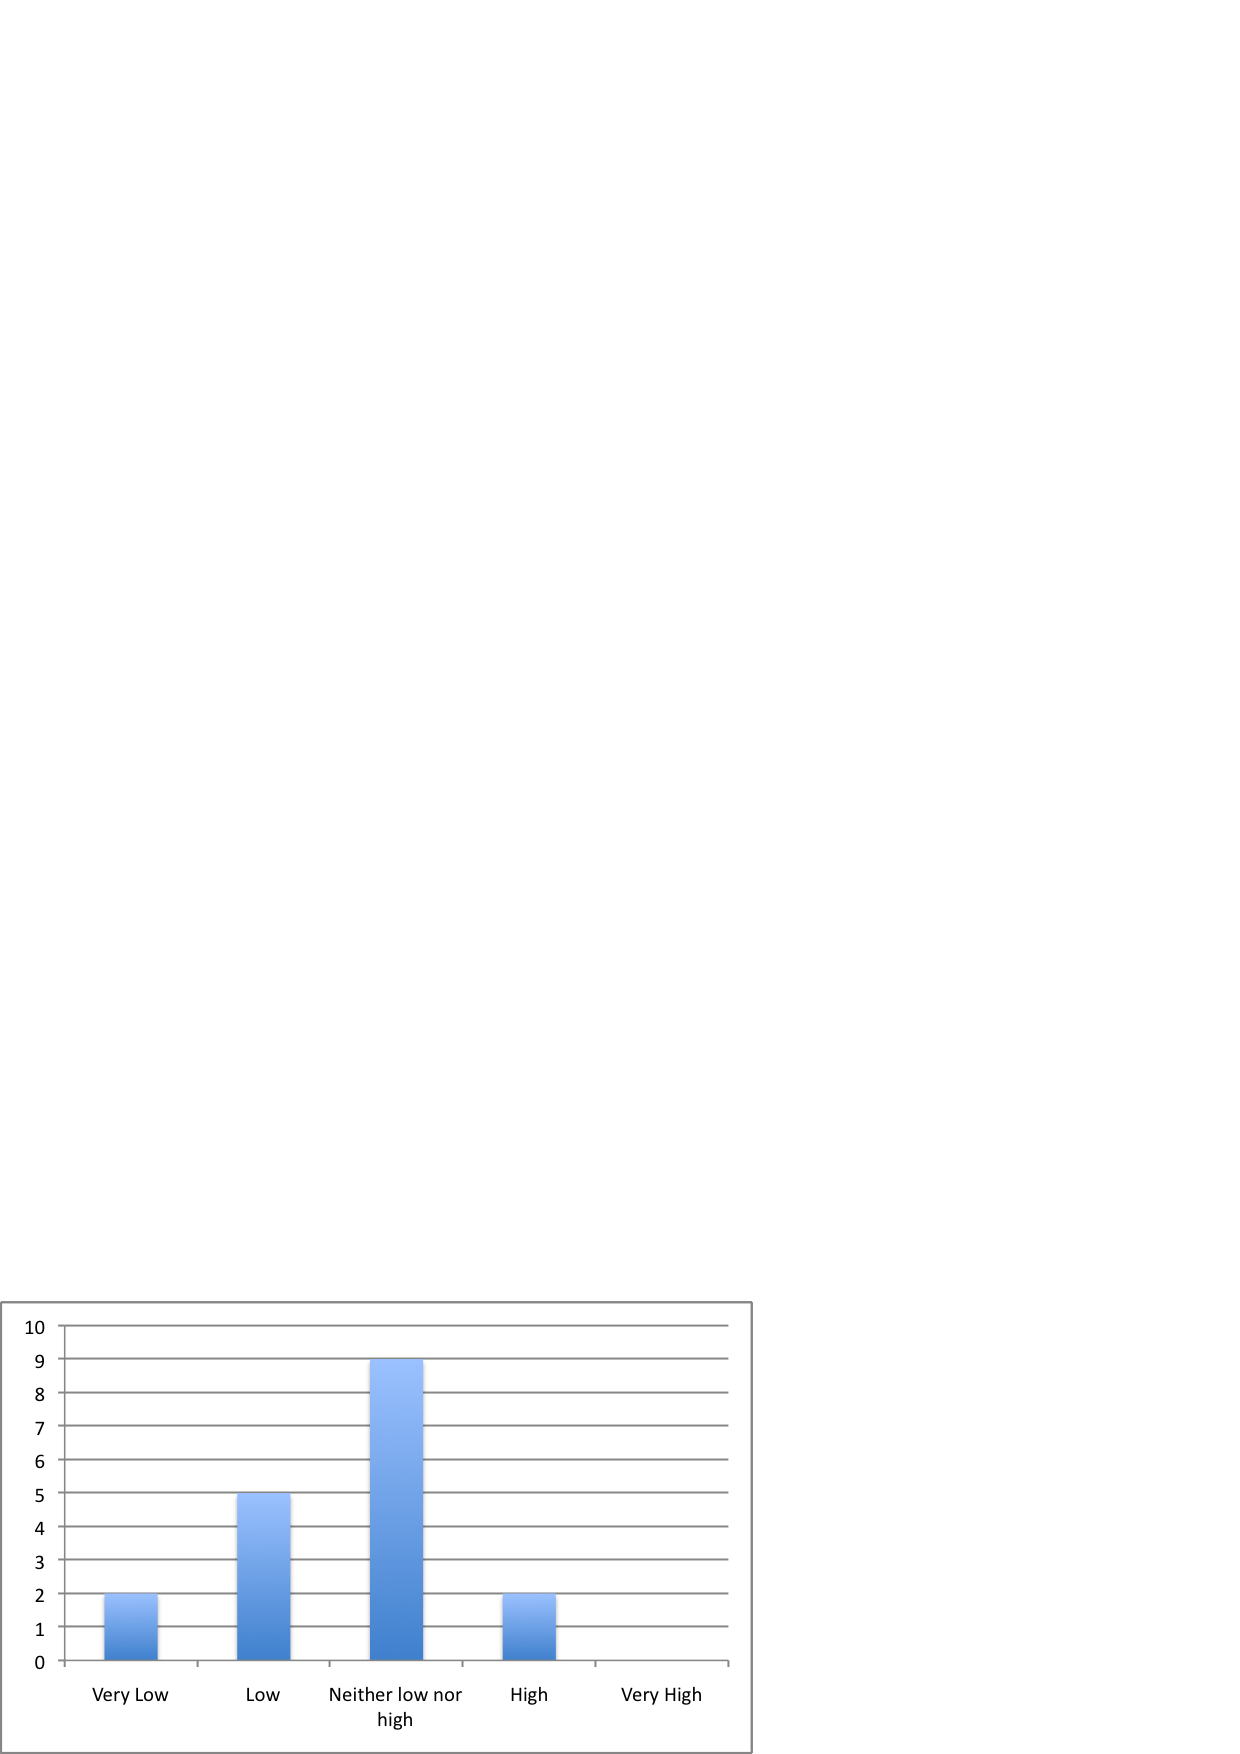
\includegraphics[width=0.6\textwidth]{Q05-AnalysisOverhead} \\ \hline

\end{longtable}
\end{center}


6. Please provide any feedback you can on Hackystat overhead, 
as well as any suggestions you have to reduce the overhead 
in future. 
\begin{itemize}
\item Since the verify command runs all the tests, I'd think that it should send data for all tests run.  Rather, in the portfolio analysis, the Unit Test portion only retrieved data for any JUnit builds that were run.  It doesn't really make sense why we'd have to run it separately when verify does it anyway.
\item If I am correct, overhead - the processing time required by a device prior to the execution of a command.  Then it all depends on what computer the user is using,  I am using a single-core processor laptop it did not take long.
\item Since Dr. Johnson provided us with Ant sensor examples, it was quite easy to set up everything to send data to the sensorbase. I did the hackystat tutorial and everything worked fine. However, I missed the part about creating a usermap.xml file for the svn sensors through Ant. That confused me a bit later on but I figured it out.

What made getting data quite easy as well was having Hudson installed on a dedicated continuous integration server. Daily builds would auto-send data to Hackystat and this made it super easy to get daily info.
\item The sensors ran automatically and it was fast with sending the data.
\item Maybe there can be a link on http://dasha.ics.hawaii.edu to both the Hudson and Hackystat server, that way we don't have to memorize the port numbers. Also, allowing us to create an account and password would go a long way towards usability. I had to put the Hackystat login information in a text file because I can't remember a randomly-generated string for the password.
\item Sending sensor data was often quite slow.  Generating reports in the web application was sometimes also slow -- the page wouldn't load until you refreshed it.
\item The overhead to collect data was generally small, however long enough that would generally run multiple (DOS) terminals so that I could continue working while it was sending data.  Analysis was no overhead since that was just pulling up a browser page.
\item When sending hackystat data, it was faily quick on my computer, MacBook Pro. Tho, there were some students I saw which had a LONG wait time on the same laptop.
\item I love Hackystat! It is a very great tool especially for a developer like me.
\item Since Ant takes care of running Hackystat sensors, this made it very easy to accomplish. 
\end{itemize}

7. Did you encounter any problems while collecting data? Was 
there any kind of data that you failed to collect? If yes, 
please explain. 
\begin{itemize}
\item I had a problem with sending commit data to hackystat when I worked on a group project. That was because I did not update my sensers to newer version. 
\item At first during the implementation of DueDates 2.0, it was not collecting commit data from my account. It was due to the account on hackystat, it included the @gmail.com part of my gmail account. So it was not matching up with each other, the hackystat account and my gmail account.
\item Running an analyses on my machine was slow, it would take over 3 minutes to run a build.  I am not sure why it took so long to send the build data so I can't make a suggestion.
\item Only JUnit data as mentioned previously.
\item Case sensitivity was an issue at first, but it was corrected so I did not get problems after that.  Hudson did not send to Hackystat number of commits, but that was fixed after a little modification with build.xml file.   
\item I was lucky. I rarely had any problems collecting data during all the time I worked with Hackystat. The one time something got screwed up was with my development time for one day. It said 0 when I checked and I had put in a bunch of time that day so it should have said otherwise. 

I don't remember exactly but, that night I believe had worked in eclipse till after 12 at night, so it went to the next day before I closed the program. That could possibly be a reason for the missing data initially. The next day I just cleared the cache and it was all fine.
\item There was a small issue when I first started collecting data, but it was quickly corrected when checking the xml files.
\item Personally I ran into no problems collecting data.
\item Sometimes it didn't collect build data for some reason.
\item Occasional problems with SVN collection, I think, was a bit hard to tell.
\item Everything was great except collecting data for my BUILD (please refer to above statement for more detailed problem regarding this). Thank you.
\item I did with commit records but it was my fault.  I wish subversion with Google Project Hosting would be more strict.  I was able to check out the project with or without the "@gmail.com" suffix (i.e. "test" and "test@gmail.com").  Thus making me two different authors.
\item Yes, the build data.  I needed to set more environmental variables. 
\item For some unknown reason, my user name picked up the @gmail.com, so both my user name with and without @gmail.com needed to be added to the projects.
\end{itemize}

8. How did you feel about sharing your software development 
data with other members of the class? 
\begin{itemize}
\item We could see how other groups were doing by sharing our software development data with other people. We also could find out what kinds of problems with our project by comparing graphs with other gropus and this helped a lot. 
\item I was not offended if it was low, and was quite intrigued with others data.  
\item I did not have a problem with sharing data with other people in class.  I thought it was needed tool to keep tabs on everyone to assure they're doing their fair share.
\item It felt good if your data was better than others.  And if it wasn't, then you felt bad.
\item Did not really like it because it is showing my programming habits, like starting on a project on the last couple of days.
\item I felt alright about sharing my data with the class. It was interesting for me to see how other people worked on stuff. Some were consistent and others were not. Some people spend a lot of time working on stuff yet do not commit as much as others that work half the time. I think its good to see this data.
\item I am okay with sharing my data.  
\item I didn't think it was a particularly good idea because it then forces group members to become competitive with each other, especially if one person is able to put in more time than all the others. Also, the data doesn't reflect the amount of work put in, maybe someone spent 5 hours doing research and only 1 hour programming, but the sensor data will only show 1 hour of development time and a minor code commit, versus someone who, say, just changes around the package structure for 3 hours and has a huge commit amount.
\item Actually hackstat (or hacky-stalk as what my teammates and I called it) caused a lot of arguments and trash talk.  Some guys were more concerned about collecting stats on hackystat than actually finishing the project.  Some members would start competing on who had more commits or move development time.  The project turned out to be more of a competition of stats, which wasn't healthy for the team at all.
\item It will be obvious that who worked on the project, so it is nice in terms of grading students. At the same time I feel some pressure that I need to work on the development, so if team leader require everybody to work well, this is good.
\item Didn't really care.
\item I had no problem with this, and it encouraged me to be aware of my time management and coding style.
\item It was good in a sense that they can help you with test cases and coverage.
\item It was fun..because you can see how everyone is doing within your group.
\item Before taking this class, I didn't think that there was a way to track software development process. After learning about software continuous integration and working in a larger group project, I have a better insight in sharing the development process. I feel that it is a must in every software development environment, big or small to be able to communicate frequently and effectively. 
\item I was nervous because certain individual of the class seemed able to put in ridiculous long hours.  I was concerned my amount of time (which seemed reasonable) would make me look as though I'm not working as hard. 
\item Good, I can see how I and others rank with each other.
\item I am fine with this.  All group projects in all schools (e.g., Architecture) should be required to use such a system.  This is great for facilitating fair evaluations of students who participate, and those who 'get the grade' by riding on the laurels, blood, sweat, and tears of others.
\end{itemize}

\begin{center}
\footnotesize
\begin{longtable}{|m{0.4\textwidth}|m{0.6\textwidth}|}
\hline 
{\bf Question}&{\bf Response}\endhead \hline
9. How frequently did you use the telemetry page? *
\begin{itemize}
\item Every day or more
\item 2-3 times a week
\item Once a week
\item Less than once a week
\item Never
\end{itemize}
&
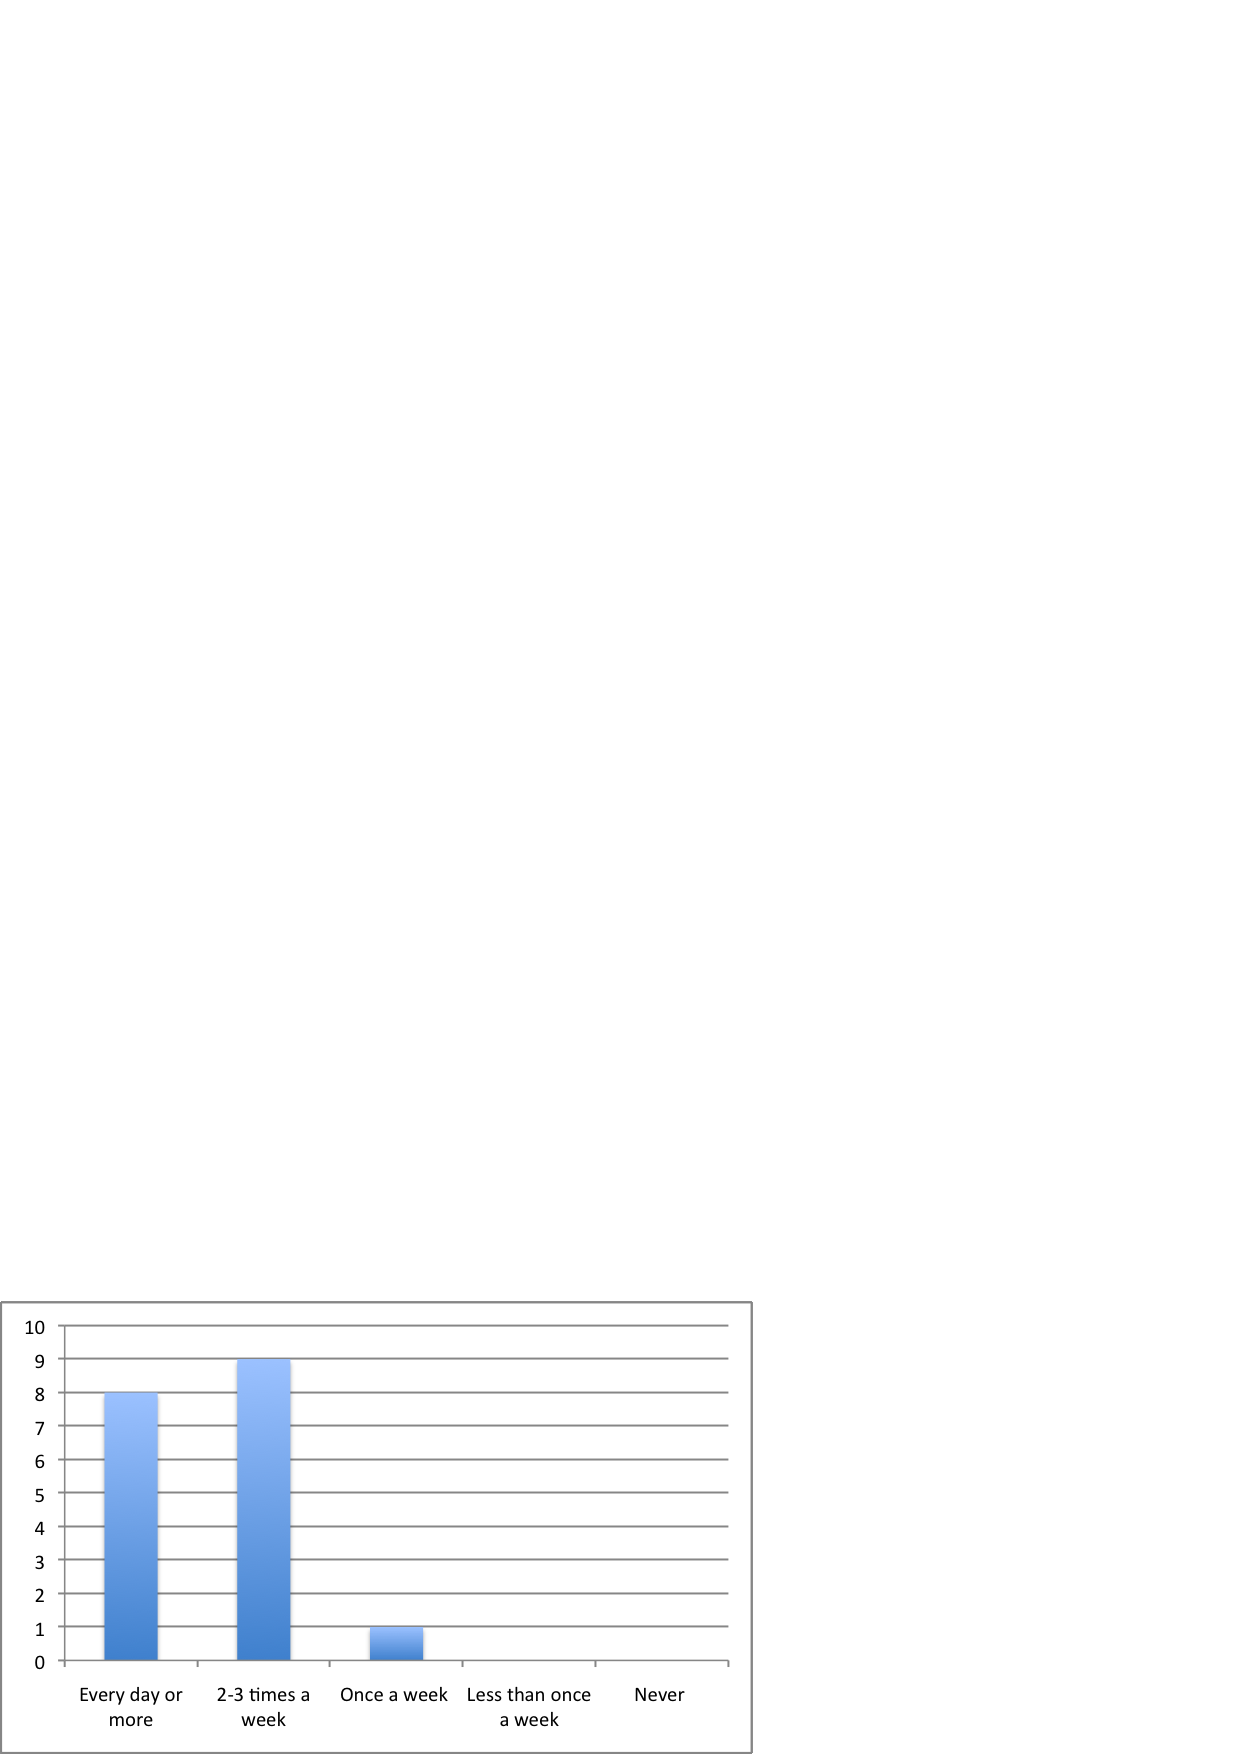
\includegraphics[width=0.6\textwidth]{Q09-telemetryFrequence} \\ \hline

\end{longtable}
\end{center}

10. If you used the Telemetry page, what were you trying to find out? 
\begin{itemize}
\item I tried to find out how was I doing for the project by looking hackystat datas. 
\item Seeing how much time i spent on the developement of the program, and also others in my group.  
\item When I used the telemetry page I was trying to find out if I was on par with other groups members in terms of development, build, and commit numbers.
\item Whether or not, my sensors were reading, and the work output of my group members (especially on days we didn't meet together).
\item If my development time was up to par with my team members.
\item I usually used the telemetry page to evaluate how my team was working overall, and what my part was in that data. I also checked it to make sure everyones data was being sent.
\item It helps me see how I measure up with my partners.
\item Member dev time mostly, to compare the amount of development time I put in vs. my group members.
\item It supposed to show us how healthy individuals are in the group. So if one person is slacking, the members need to tell him to step it up.  It wasn't used that way in our group.  One person really wanted a good grade for the class so he just used the telemetry to watch himself; making sure no one gets more builds/devTime/commits than him (yes he said ``i need more dev time because i need an A'').  I remember we had dinner as a group and one of our group members didnt go to dinner.  another group members then said ``oh if he ups his stats more than mine, tomorrow im gonna hack all day.''

Sad, but true.
\item member commit, member dev time
\item Curious about trends in dev time, commits.
\item Usually MemberDevTime, MemberBuilds, and MemberCommits.  Basically just seeing how everyone was progressing.
\item graphs, line trends of other group members
\item My status and the status of our group and make sure everyone is doing their part.
\item Mostly trends in individual performance, as well as overall project outlook.
\item Basically if everyone was putting in the same amount of effort.  Also it helped indicate if everyone is on track.  If they have regular activity, then the chances of them on track is higher.  
\item Was the coverage, complexity and coupling getting bad?
\item I tried to review each telemetry page daily to understand what I could do to improve the project health and focus efforts.
\end{itemize}

\begin{center}
\footnotesize
\begin{longtable}{|m{0.4\textwidth}|m{0.6\textwidth}|}
\hline 
{\bf Question}&{\bf Response}\endhead \hline
11. How frequently did you use the Software ICU? *
\begin{itemize}
\item Every day or more
\item 2-3 times a week
\item Once a week
\item Less than once a week
\item Never
\end{itemize}
&
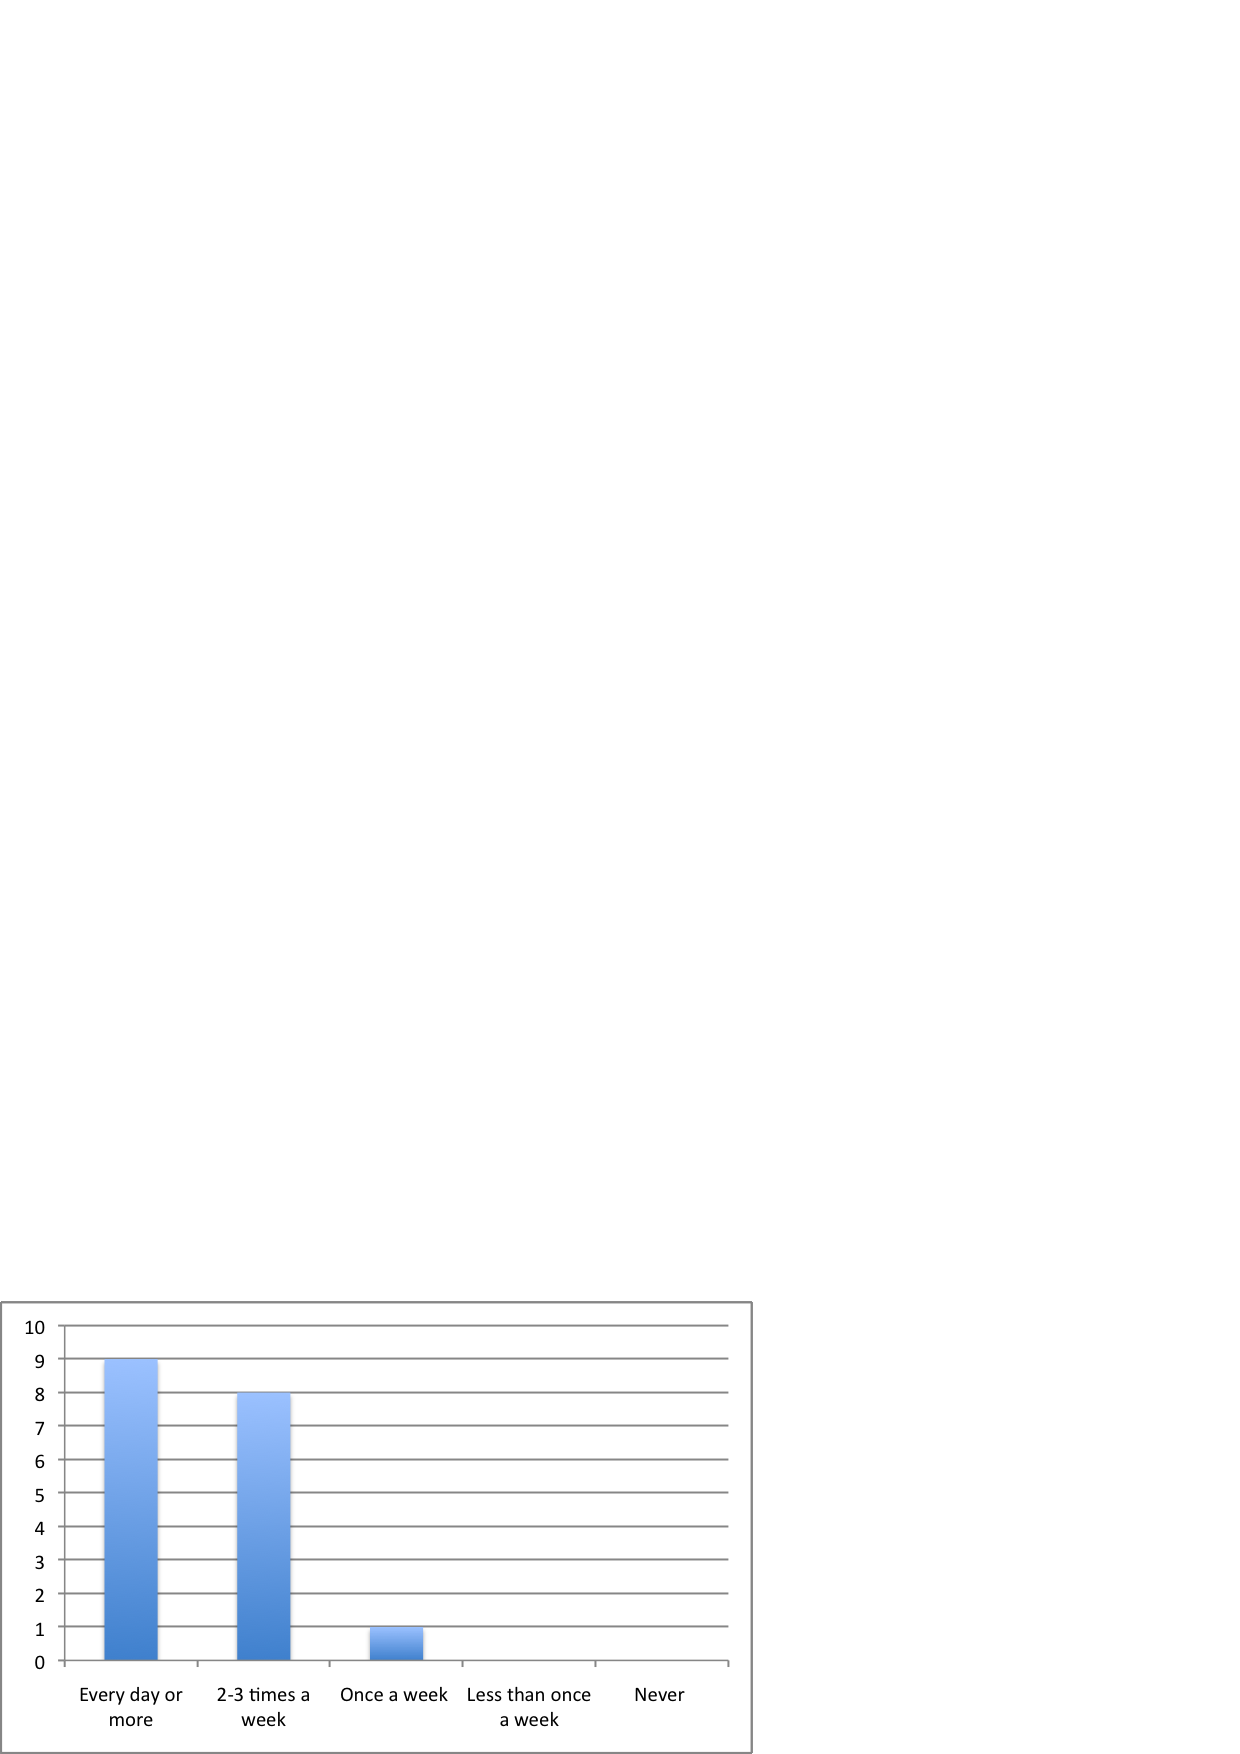
\includegraphics[width=0.6\textwidth]{Q11-ICUFrequence} \\ \hline

12. If you used the Software ICU, please check the vital signs that were useful to you. *
\begin{itemize}
\item Coverage
\item Complexity
\item Coupling
\item Churn
\item Size
\item DevTime
\item Commit
\item Build
\item Test
\item None of the above
\end{itemize}
&
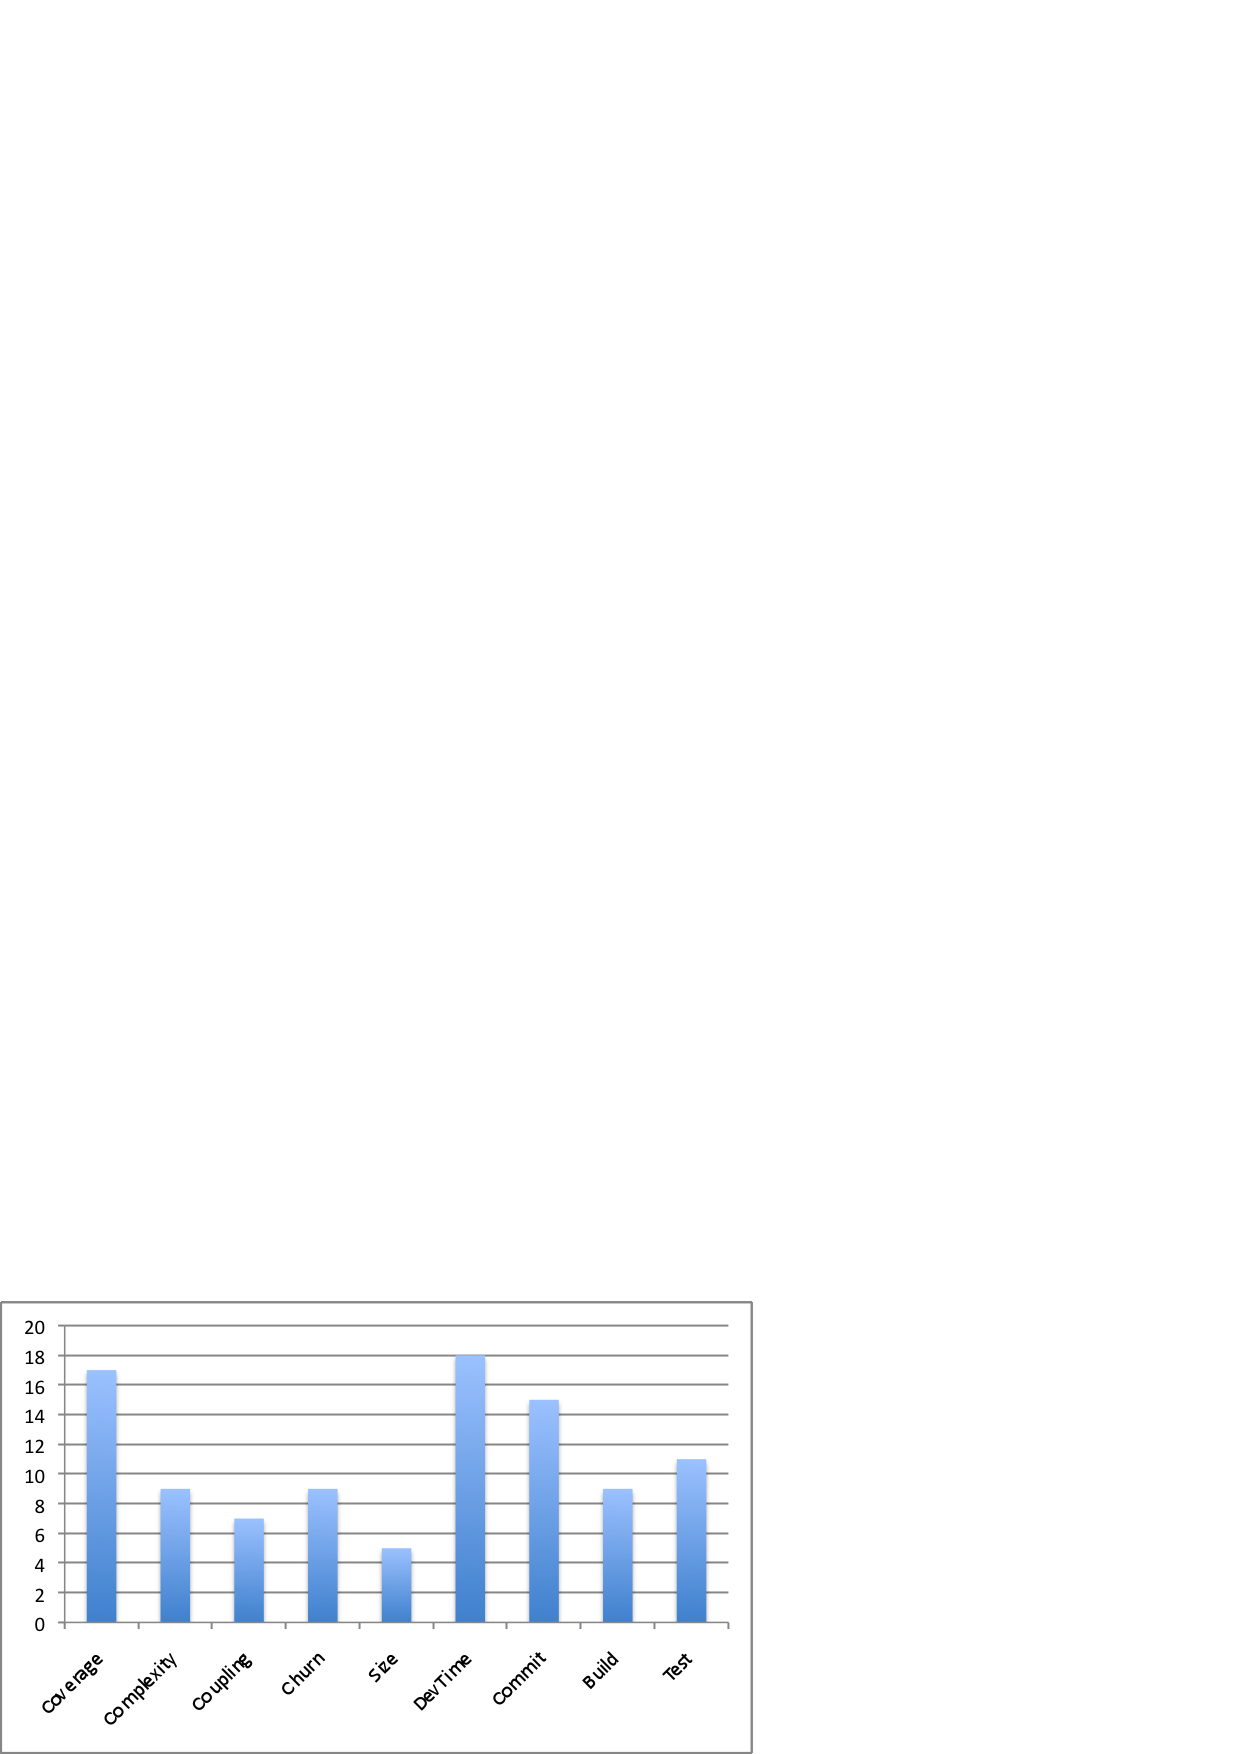
\includegraphics[width=0.6\textwidth]{Q12-UsefulVitalSigns} \\ \hline

\end{longtable}
\end{center}

13. Did you feel the Software ICU colors accurately reflected the health of your project? If not, why not? 
\begin{itemize}
\item I felt most of colors accurately reflected the health of the project. For the Coverage datas, since we can write test cases just for incresing of the rates, we cannot assume that the project is in healthy condition even if the coverage datas displayed in green color. However, I think this is not a problem of hackystat. 
\item Yes
\item The only issue I had with the ICU colors was with the coupling.  In both versions of DueDates we had to add extra classes at the last minute which would cause the coupling ICU to turn red.  I am not sure how to address that because the coupling does need tracking.
\item Not really, I don't think having a high churn amount is necessarily bad.  Of course, it's a case-by-case thing.  For my group, it wasn't about not committing frequently; we were just rehashing code because something just didn't work.
\item Yes, reflected accurately on the health of the project.  Showed how much coverage we had.
\item I feel that the Software ICU did accurately reflect the health of my projects. For Due Dates 2.0, which was a longer project, the data was getting increasingly more meaningful as the trends were over a larger period of time. It is good to look at things like devtime, commits, coupling, and coverage to see the color and the past trend because i think they really say something about the current state of the project.

To make it simpler, whenever I knew our project wasn't doing good and people weren't working regularly, the software ICU would have lots of reds and yellows. When I knew the project was doing better and people were working regularly, there were greens. It makes sense.
\item The ICU was accurate with our project because it showed drastic spikes in all signs.  This reflects our project in poor health.
\item Not particularly because a project's health cannot easily be determined by just measuring numbers alone. For example, it's easy to increase coverage, but if a class has nothing but getters and setters and a toString method, does it really need to be tested? Of course not, but someone might feel compelled to do it in order to increase coverage and get a better health, but it's just a waste of time in my opinion. Also, DevTime is only measured from Eclipse but that doesn't measure things such as someone reading a book or looking up websites for information. It only measures active development in one program, forcing people to only use whatever IDE's Hackystat supports. The figures for complexity and coupling are hard to evaluate too. We want complexity to be low but sometimes it's unavoidable for it to be high, and should Hackystat show an absolute cut-off point where the complexity must be below a certain point for the project to be considered acceptable? Coupling is another one that falls under this category, if your program relies on a lot of outside libraries, can someone really determine an absolute value that the project's coupling must be under?
\item Yes.
\item maybe
\item Coverage: perhaps too sensitive to drops/bounces in coverage.
Churn: while you're working on a project, churn is going to vary, sometimes a lot.  The trend colors were not helpful.
\item Yes, I felt it was a relatively healthy project, and this generally showed, in the end.  In the first half the colors reflected not as health of a project, which I'd agree as well.  I'm not sure rising coupling was entirely a bad sign as things went along and functionality was added, as it was a slow steady rise.
\item Sometimes.  Hard to determine what will fall into green, red, or yellow.
\item Yes definitely.
\item It somewhat reflected the quality of our project. Maybe in some dark corner something is not thoroughly being depicted through the colors. Perhaps a suggestion is to use different color hues.
\item Yes it was pretty accurately reflected.
\item No, since I did not correctly configure the sensors.
\item This is subjective...  Usually the colors were spot on, however, they are quick to turn one way or the other depending on events that are being managed by the team (e.g., large code churns due to removal of unused code/imported code, etc.).
\end{itemize}

14. Were you able to use the Software ICU to improve your software's quality and/or your team's process? If so, in what ways? If not, why not? 
\begin{itemize}
\item We can check how other members are doing for the project through the Software ICU and this helps a lot especially when we are working on the team project. 
\item Yes, for tracking if members were working on their tasks. Also how complex the program is increasing or decreasing. 
\item In my opinion, it is not clear if the ICU improved our system.  Because other tools such as junit, findbugs, and pmd was easier to use to improve the application.
\item If anything, keeping an eye on coverage helped us look out for what was being tested and what wasn't.
Yes, showed how much coverage we had, and improve on that.
\item I think for sure the Software ICU improves team process. Moreso than just keeping people ``in check'' when grades are at stake, it provides an accurate way to assess what's being done and by whom. Our team got a lot out of checking up on the software ICU and assessing our team process. It seemed to get better over time.

As far as the software's quality, I think the Software ICU could be very useful in improving this. If my project for instance was in the red for complexity and coupling, and there were some code issues, I could see all this automatically through hackystat. Besides coverage stats though, my team did not really use the ICU to improve the software's quality.
\item ICU was able to help us because it told us what needs to be focused or corrected.
\item Personally, I only found Hudson useful because it's like running your code on someone else's computer to see if your environment is set up differently from a generic machine. I feel that the data for Hackystat is more something to look at out of curiosity rather than something to determine how well a project's status is because it's hard to base a project's health based on numbers alone and it might put unrealistic pressures on the team to make the project healthy for Hackystat when they can better spend their time developing instead.
\item Yes.
\item Yes, coverage tells me if we didn't write enough test cases.
\item No.  
Coverage: already aware from Emma.  
DevTime, Commit, Build, Test: either team members did not look at the statistics, or they didn't care, because their habits did not change much.
Others: not much we could do about the other statistics.
\item Yes because able to manage our time and development fairly equally, and also notice spikes indicating bigger changes or problems.
\item Yes, shows were we could improve as a group and improve as a programmer.
\item Like in my case last time, I saw on Software ICU that I don't have a data on my BUILD. So because of that information I know what the problem is and it helped me to find a solution and figure everything out before it is too late.
\item Our project ICU definitely described our lacking and late attempt to improve coverage. Due to the ICU, we were able to distinguish this fact quick and easy. 
\item The amount of activity helped us identify who was falling behind.  Without offending our members by outrageously claiming their not working, we could tell by the sensors.  Members can be more self-critical by looking at their individual data compared to the groups.
\item Yes, by checking the coverage, complexity and coupling.
\item Yes.  By targeting coverage, dev time, coupling, and complexity, my team was able to improve all these into areas that were acceptable to us.
\end{itemize}

15. Please provide any other feedback you would like regarding 
Telemetry and the Software ICU, as well as any suggestions 
you have on how we can improve the system. 
\begin{itemize}
\item I do not think the commits, builds, tests should be colored in because it all depends on how much the user does on the project.  Is it possible to show line coverage instead of method coverage? The software ICU and telemetry was awesome tools in helping out with the project.  It gave me visual stats on the project.
\item What I think would be cool is to implement something to view the trend for each category in larger format but in the same style as the software ICU. I know this is shown on the telemetry page when you select it to show. However, I would be nice if there was some sort of rollover function that brought up a slightly larger window with a blown up overall trend. I can see how this isn't really needed but I would mostly likely check it a lot if it was there. 

A minor thing that I noticed when using the Telemetry page was that when I selected a new statistic to view, the page would always jump back to the top and I'd have to scroll down each time. Its not really a biggie, but it makes navigating a bit slower when your going through all the project statistics.
\item Consistent colors for each members can help.
\item In addition to everything I mentioned above, it might help to somehow make the sensors configurable in some way, for example if two people are doing pair programming, there should be an option to set the sensors to send data for both people. Perhaps complexity can be measured somehow to only include methods that, say, start with get or set and toString. This way people aren't forced to write pointless test cases in order to increase coverage. 
\item Help page should be provided inside project browser. It should describe how to use it, what telemetry, what churn is, something like that. 

Also your explanation should be simple so that people want to read it. If it is complicated and long explanation, nobody will read it. 
\item The different color bars and randomness might be fun and interesting, but I think having a bit more consistent scheme might be better.  I would suggest if possible giving each developer a specific color that they always have during the project, either random, or choosen at the beginning.
\item Does not capture development outside of Eclipse.  For example, IMHO, MS Visual Studio is much better in the capacity as a web development IDE, which the dev time here was not recorded.
\end{itemize}


\begin{center}
\footnotesize
\begin{longtable}{|m{0.4\textwidth}|m{0.6\textwidth}|}
\hline 
{\bf Question}&{\bf Response}\endhead \hline
16. If I was a professional software developer, using Hackystat at my job would be: *
\begin{itemize}
\item Very feasible
\item Somewhat feasible
\item Neither feasible nor infeasible
\item Somewhat infeasible
\item Very infeasible
\end{itemize}
&
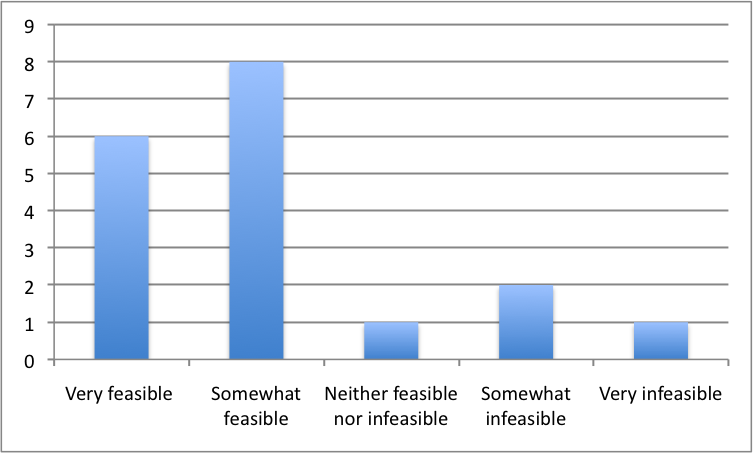
\includegraphics[width=0.6\textwidth]{Q16-FuturePredict} \\ \hline

\end{longtable}
\end{center}

17. Please provide any other feedback you can on the feasibility of Hackystat in a professional setting, as well as any suggestions you have on how its feasibility could be improved.
\begin{itemize}
\item I think its good to have this in a professional environment, cause the employer or client  can check on how the progress of the program is going. With out having to make so much visits or hovering over workers.
\item Cannot think of any off of my head.  The Software ICU is already great for us programming students.  
\item I think Hackystat is definitely feasible in a professional setting, as long as it is supported in some way. For instance, if a team of developers is working on a project and they are all for having Hackystat manage project stats, that would be great. If, however, your the only person on your team that wants to use it, then it would be hard to send data that would assess team process.

I could see project managers wanting to have Hackystat data to evaluate everyone's input into the project, as well as the health of the project. Hackystat, I think, is perfect for new open source projects if releases are made early and often. It could be essential to seeing the overall health of the project.
\item Overall, I feel like Hackystat would be an interesting tool to gather data to look at for curiosity's sake from time to time, but it should not be used as a basis for determining a project's health or to determine something such as member contribution. The sensors can only gather information from a few sources and these readings cannot account for a person's full contributions to a project. As for determining a project's health, I do not believe the sensor readings can provide an accurate measurement because the sensors can only measure numbers based on algorithms, but it takes a person to really determine how good the code is.
\item When I start to use hackystat, I need to get password from you and then eclipse send my data to your server. Some developers might have concern that hackystat steal source code.
\item I think it depends a lot on the culture of job setting.  I'm not too sure, but I think I may try setting it up on my own job site, even if just for myself to see my own trends.
\item It is a very useful tool to keep track the health of a project so I would say it is feasible to have it in a job.
\item My only wish is that ICU's should have a feature to support pair programming. Possibly a feature to indicate to the system that two people may be working on the same problem on the same system, rather than two individual machines. You might want to call this "collaborative mode," or something along the lines of that. These settings of course should be turned on or off easily from the developer's IDE (Eclipse).  
\item I work in a one person shop, so it would be difficult to say how useful this would be.  As a lone developer, many metrics I am very cognizant of, however, having such a system would allow me to view those statistics that I do not have a "gut" feeling for.  It would be great for my boss to measure the amount of time I spend on a project however.
\end{itemize}
   
\section{Interpretation of the 2008 data}
\subsection {Experimental Limitations}

Before drawing any conclusions from this data, it is important to recognize the limitations of this study. Compared to the limitations associated with previous study in 2003 and 2006, anonymity is achieved, but others are still unsolved in class evaluation.

First, this data is drawn from a limited sample size of 18 students in software engineering classes at the University of Hawaii. The subjects therefore have a relatively narrow and homogeneous background in software development.

Second, the context in which they used the system was a course project.  Course projects tend to be smaller, narrower in scope, and with less pressure on the developers than an industrial context.  It is one thing to get a poor grade for doing a poor job, it is another thing to lose your job for doing a poor job.  In addition, students are not working full-time on the system; the development project is just one assignment among several.  

These are all major limitations on the external validity of the responses.  They do not make the results meaningless, but rather help provide a perspective on how to gain additional evidence in future that would confirm/disconfirm these initial findings.  For example, it would be helpful to deploy Hackystat in a real software company, and then gather data anonymously from the coders and managers. Other insights into future research directions will be covered in an upcoming section.

\subsection {Conclusions regarding Installation/Configuration}
The data indicates that eclipse sensor was easy to install. To install Ant sensors were a little more difficult. The most difficult one is the SVN sensor, which require configuring Hudson, a continuous integration engine. 

Major installation difficulties is the documentation. Though we provided guides for every component, some students point out that the documentation is too distributed and too long. Some guides are too similar that slightly but important difference will be easier ignored. A more straightforward and brief walkthrough or even an auto installation package are most expected.

Regarding the collection of data, no problem reported. 

The installation/configuration of Hackystat services(SensorBase, DailyProjectData, Telemetry, etc.) were not evaluated because the students were all using the public services\footnote{SensorBase: \url{http://dasha.ics.hawaii.edu:9876/sensorbase}, DailyProjectData: \url{hhttp://dasha.ics.hawaii.edu:9877/dailyprojectdata}, Telemetry: \url{http://dasha.ics.hawaii.edu:9878/telemetry}, ProjectBrowser: \url{http://dasha.ics.hawaii.edu:9879/projectbrowser}}.

\subsection {Conclusions regarding overhead of use}
The overhead of collecting data and running Hackystat analyses were neither low nor high. The comments indicate that the major concern was speed, both of collecting data and of running portfolio analysis.

\subsection {Conclusions regarding sharing development data with other members}
Most students felt OK with sharing development data with other members. But some students did have concerns that sharing development data would reveal their programming habits and introduce too much competition of statical stats, which made them nervous.

\subsection {Conclusions regarding usage and utility}

\autoref{fig:usage-compare}, \autoref{fig:usage-overtime}, \autoref{fig:metrics} and \autoref{fig: memberlevel} show the data from system usage logging. We will combine it with the data from questionnaire to gain insight into Hackystat's utility. Also while comparing these two collections of data, we verify that the data is reflecting the true properties of Hackystat.

\begin{figure}[htbp] %  figure placement: here, top, bottom, or page
   \centering
   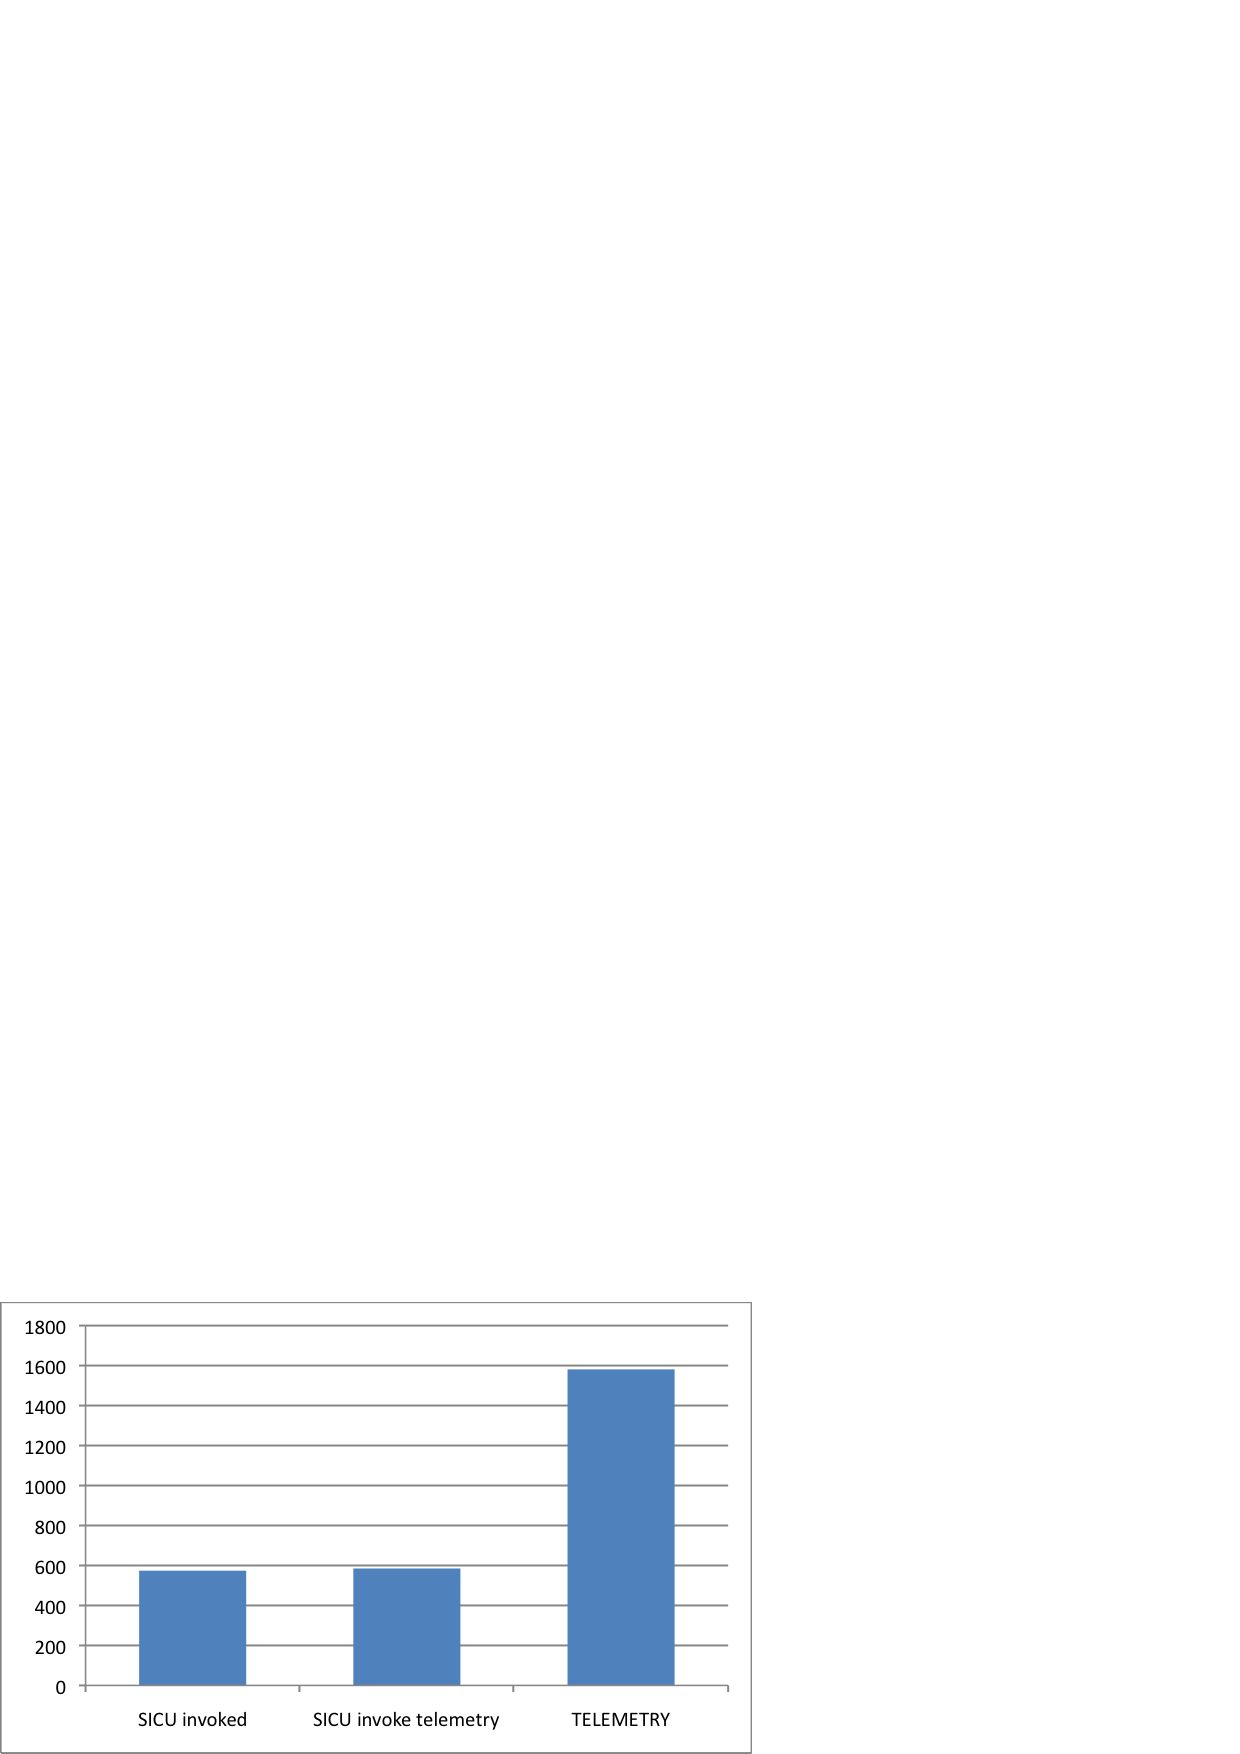
\includegraphics[height=15em]{usage-compare} 
   \caption{Usage comparison of SICU and Telemetry}
   \label{fig:usage-compare}
\end{figure}

\begin{figure}[htbp] %  figure placement: here, top, bottom, or page
   \centering
   \includegraphics[height=20em]{usage-overtime} 
   \caption{Usage trends of SICU and Telemetry over time}
   \label{fig:usage-overtime}
\end{figure}

\begin{figure}[htbp] %  figure placement: here, top, bottom, or page
   \centering
   \includegraphics[height=20em]{metrics} 
   \caption{Usage Comparison of each Telemetry analysis}
   \label{fig:metrics}
\end{figure}

\begin{figure}[htbp] %  figure placement: here, top, bottom, or page
   \centering
   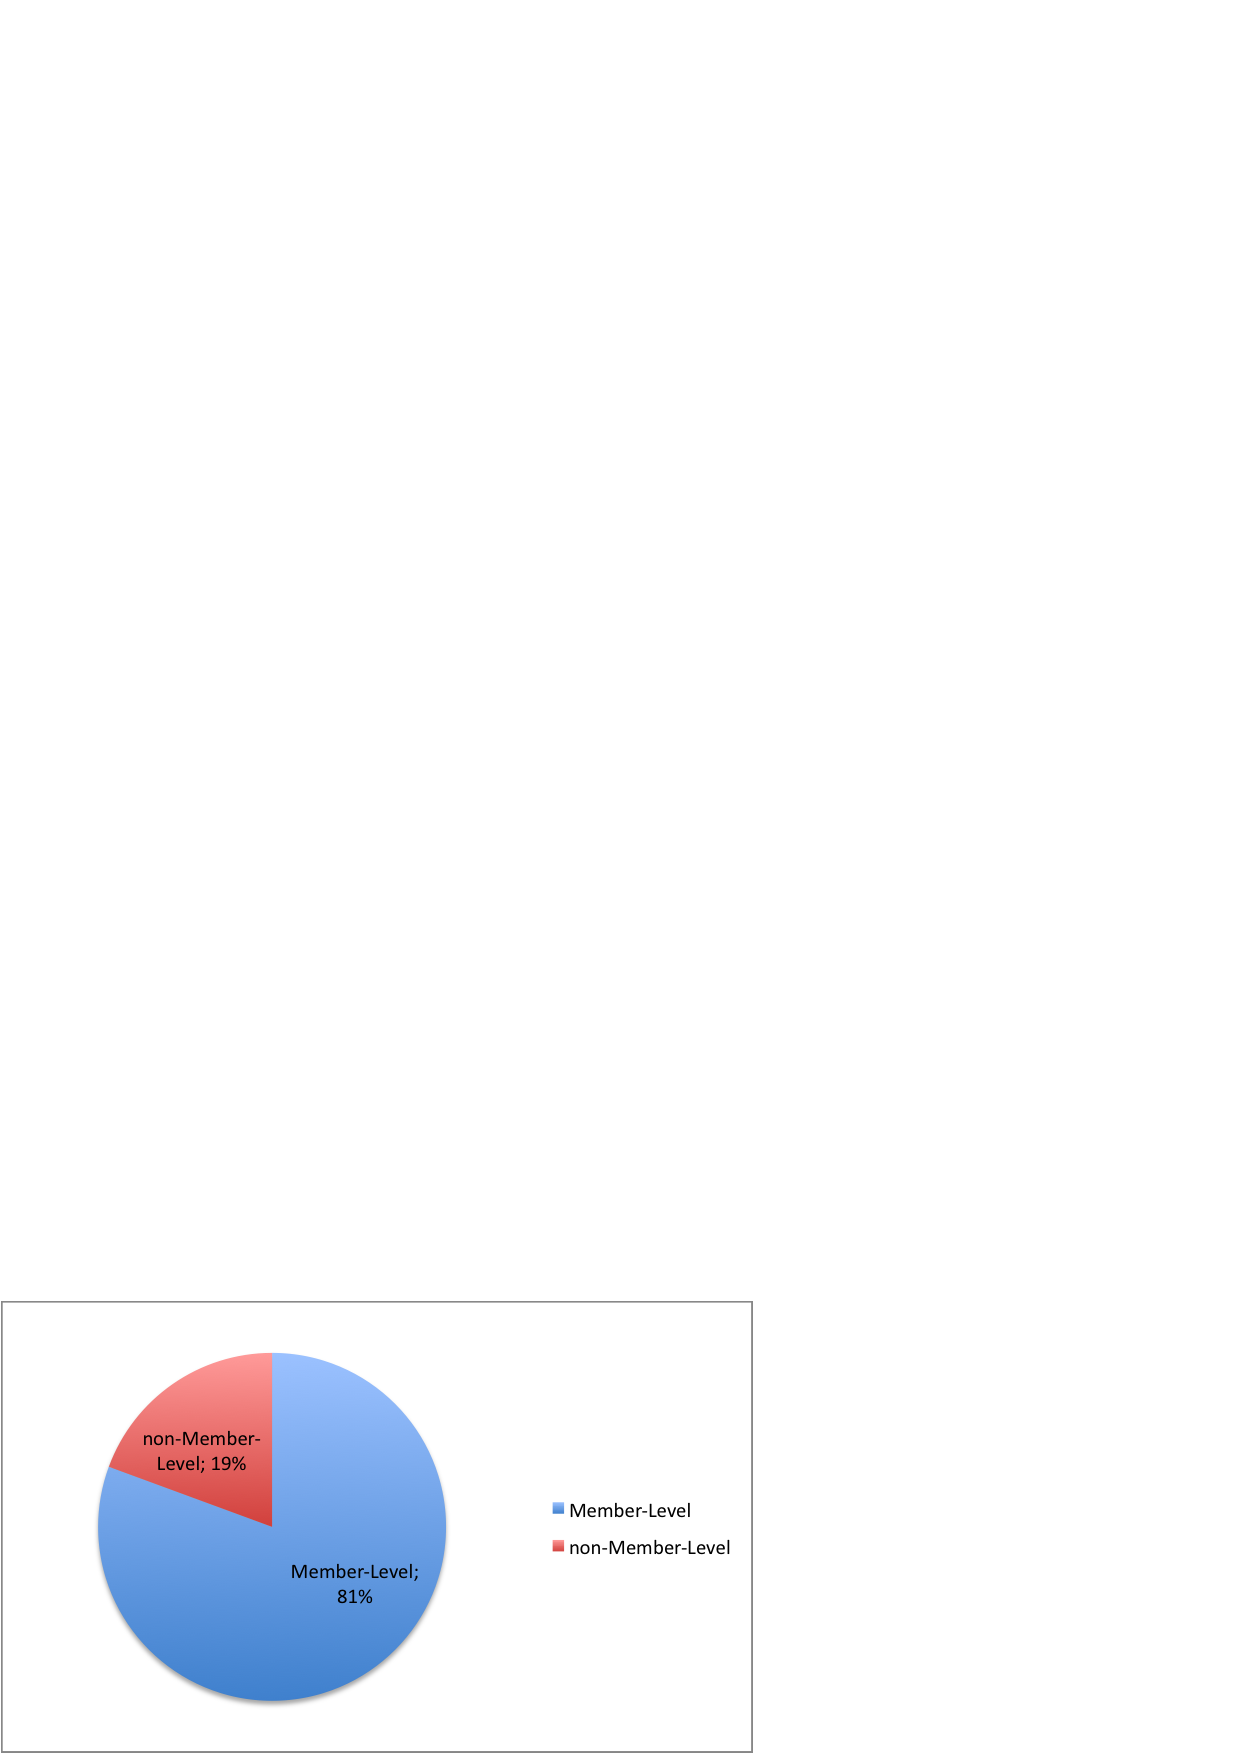
\includegraphics[height=20em]{memberlevel} 
   \caption{This figure shows that Telemetry is mainly used for member-level analyses.}
   \label{fig: memberlevel}
\end{figure}

Both data from questionnaire and system logs indicates that Telemetry and Software ICU were frequently used during the evaluation period. Telemetry is invoked much more frequently than SICU, and the frequency of invoking SICU and invoking Telemetry from SICU is similar (see \autoref{fig:usage-compare}). The variations of invoke frequencies over time are rough synchronized among these three events(see \autoref{fig:usage-overtime}).

Considering vital signs separately, popularitiy of three useful vital signs are outstanding from others according to the questionnaires. They are DevTime, Coverage and Commit. Similarly, Member DevTime and Membr Commit accounted for more than half of the usage in Telemetry analyses in system usage logs(see \autoref{fig:metrics}). These two Telemetry analyses are also the most mentioned analyses in Question 10. Responses of Software ICU accuracy indicates high attention on coverage as well. The Coverage is not of the top use in Telemetry analyses is possibly because it is enough to comprehend it from SICU, and Telemetry is mainly used for member-level analyses(see \autoref{fig: memberlevel}).

The vital sign popularity can be partially explained by the comprehensive difficulty of the vital signs. Compared to other vital signs, the three most popular analyses are more intuitive than others. DevTime and Commit are the sign of work output and it is always prefer to be higher. Coverage shows the proportion of the code that covered by unit tests, and is also higher the better. In contrast, other vital signs are some more sophisticated to make sense of. Though it is believe that Complexity and Coupling are preferred to be low, it is hard to tell what a certain number means to the health of a project. The Build and Test are only the number of Ant builds called, which did not mean either good or bad of a project or developer. Churn is the most difficult one to interpret. It shows the lines of code edited in the inquired period. Neither does high nor low necessarily indicate a good developing habit. In SICU, it is simply presented to be lower the better, which introduce confusion among students that it theoretically prohibits them from committing too much code in a day. This is another reason that Churn is not weighted as much as the popular metrics.

Although DevTime attract most attention, its accuracy is doubted. Currently DevTime is only collected from limited tools. DevTime data about work on other tools or doing research it is not collected. It makes DevTime highly inaccurate in measuring a member's work output, and thus sometime cause unhealthy competition within group partners.

Regarding Software ICU as a whole, 7 out of 9 vital signs are considered to be useful by at least half of the respondences and 10 out of 18 responses said the Software ICU was accurately reflecting the health of their project via colors. 4 responses disagree that was accurate, mainly because high and/or increasing Churn and Coupling are not necessarily bad. Most students thought Hackystat did help them improve their performance either in programming or teamwork or both.

We can conclude that, though there are still some deficiencies about presentation methods and potential bias of the data cause by its native or collection, Hackystat does achieve its goal to provide users useful tools to help them understand and improve their programming procedure.


\subsection {Feasibility in a professional software development context}
The data indicates that most students thought it was at least somewhat feasible to use Hackystat as a professional developer. Most comments indicate that Hackystat would be helpful in professional settings. There are some arguments about the potential bias of analysis data of Hackystat that the statistical data did not accurate enough to exclusively determine a project's health state.

\section{Comparison to the results of 2003 and 2006}
\subsection{Hackystat in 2008 vs. 2003 and 2006}
To usefully compare the data from 2003 and 2006 to the data from 2008, it is necessary to understand the changes that have been made to the Hackystat system since 2006.

First, in 2007, the Hackystat system underwent a complete rewritten for a new version. Hackystat now is organized as a collection of loosely coupled software services that communicate using REST architectural principles. The new architecture is much more extensible than previous versions. Upon it we built the SICU analysis, which is almost impossible in previous version because it involves large scale of data. We also built a new web interface called Project Browser, which we believe it is the best UI in Hackystat history.

Second, new sensors and metrics are introduced since 2006. Beside the seven metrics used in 2006 (Coverage, Code Issues, DevTime, Commit, Build, Unit Test, LOC), three new metrics are introduced to the evaluation: Cyclomatic Complexity(from JavaNCSS), Coupling(from DependencyFinder) and Churn(from Subversion).

Third, the main analysis used by students are changed since 2006. In 2003, the students mainly used the course project analysis that presented summaries of the individual team project to-date metric data and the comparisons of all of the course projects. In 2006, the data was presented by the Software Project Telemetry system, which show trends over time. In 2008, the Telemetry service was still available to them. Upon it and the DailyProjectData service, we built a new service called Software Intensive Care Unit(SICU) to present the data. It combined the functionalities from the systems in 2003 and 2006 that presented both to-date data and trends of the projects. The interface, which built upon Wicket, is more user-friendly and easy to interpret.

Fourth, in 2003 the students had to manually install the sensors and in 2006, they used hackyInstaller, a GUI system, to simplify client-side installation. In 2008, because of the complete re-implementation of the system, they had to manually install the sensors again.

Fifth, in 2003, the principal analysis provided a tabular representation of "to date" values for one or more of the course projects, as illustrated below:

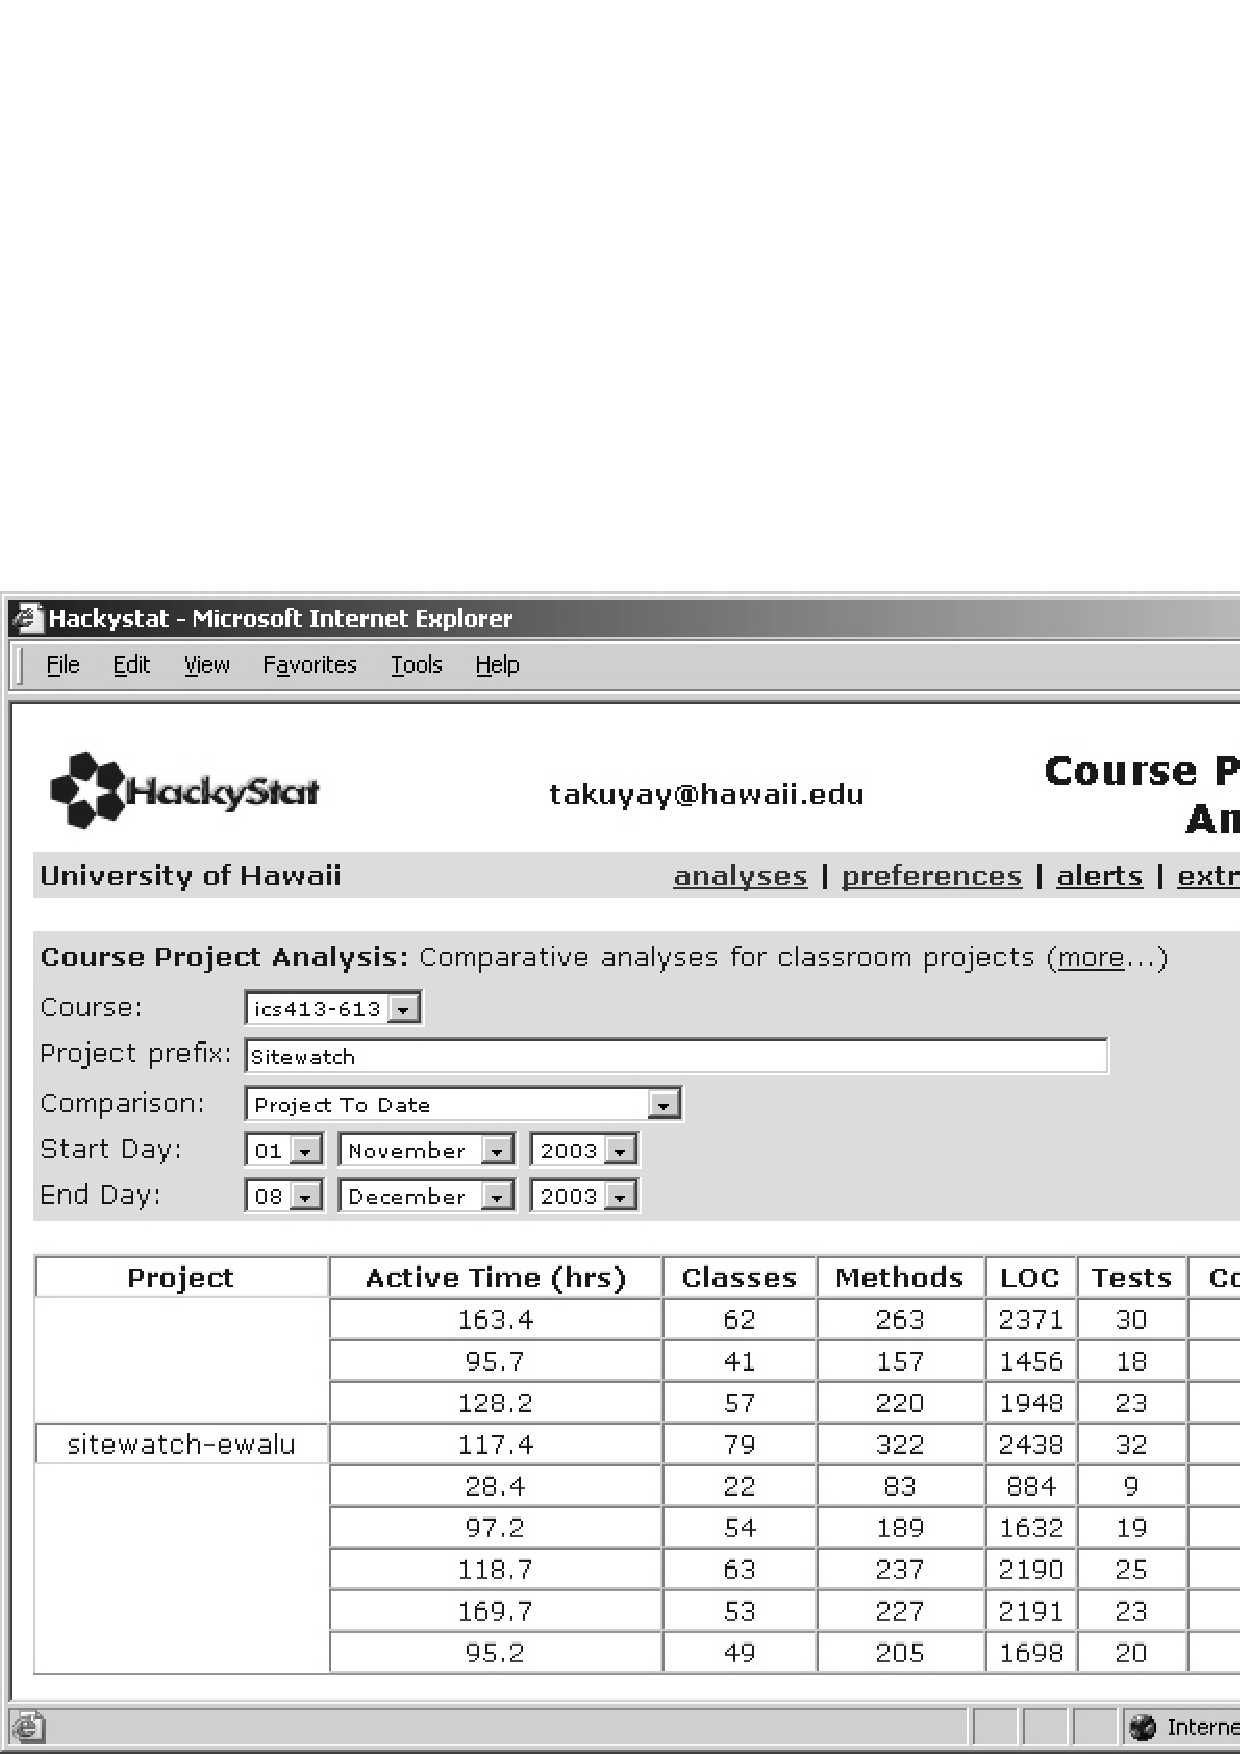
\includegraphics[width=0.8\textwidth]{course-project-analysis-to-date-2003}

In 2006, the principal analysis was based upon software project telemetry. The following image shows one of approximately a dozen different charts that the students would use to analyze and interpret their collected data:

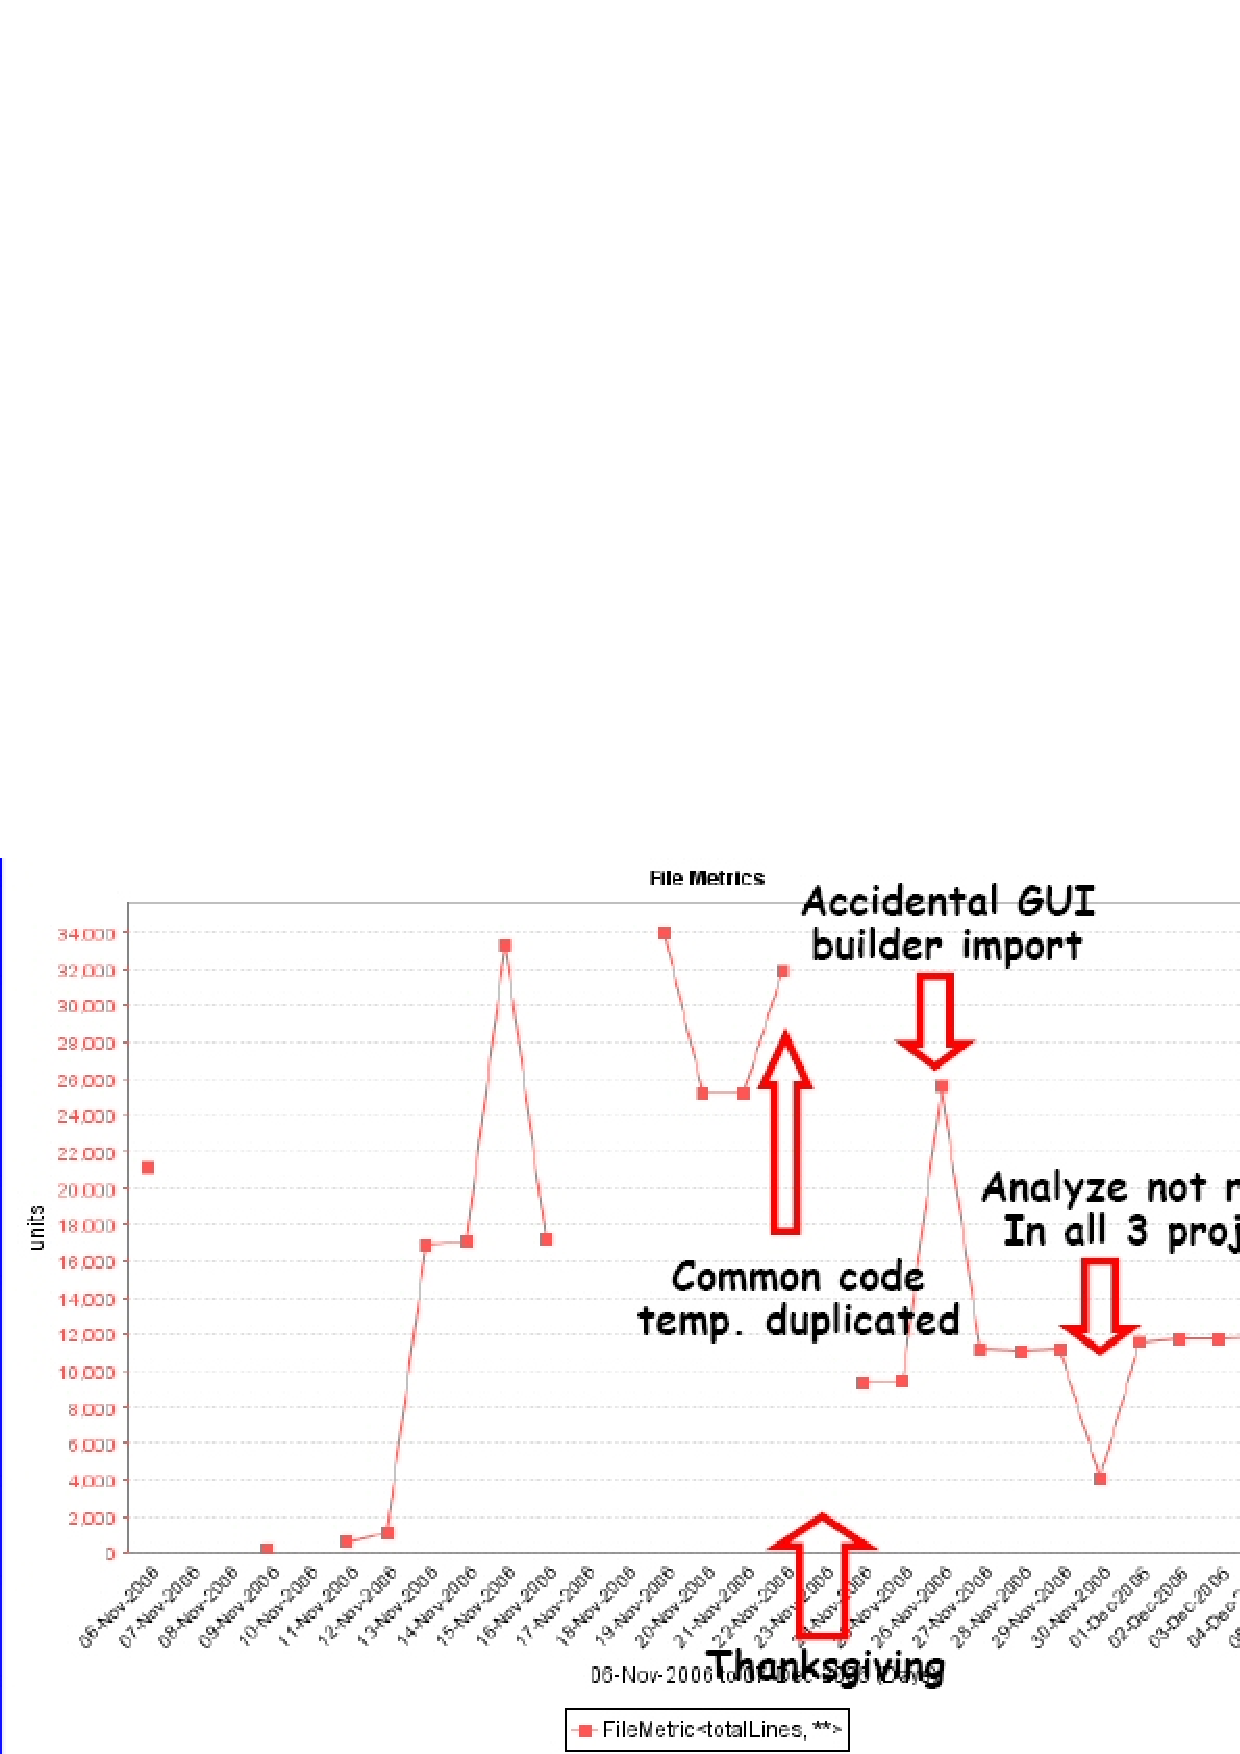
\includegraphics[width=0.8\textwidth]{telemetry-2006}

In 2008, the principal analysis was the SICU, which presented the both the to-date metric data and trends via spark-line in tabular form, as illustrated below:

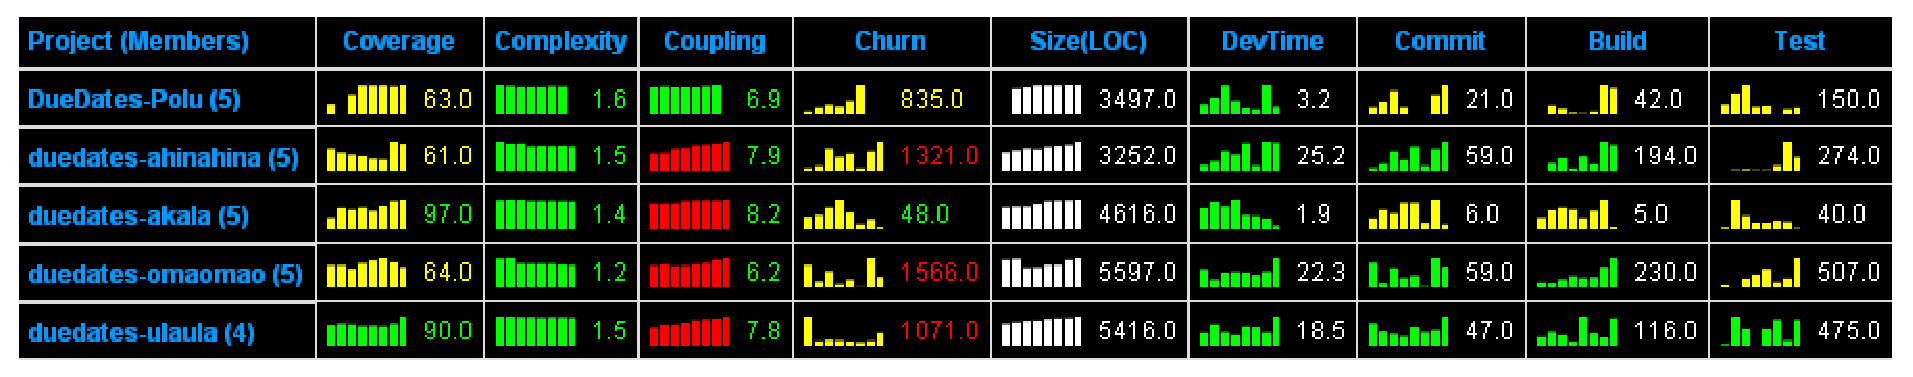
\includegraphics[width=0.95\textwidth]{portfolio-2008}

In order to facilitating the interpretation of the data, the numeric data and spark-line trends are colored according to the state it represent. Green, yellow, red mean good, average, bad. It gave user an intuition about the ``health'' state of the projects.

\subsection {Comparison of the empirical results}
The next section presents a comparison of the data from 2003, 2006 and 2008. All data has been convert to percentage in order to normalize the number of participants. Any differences claimed between the data sets based upon the ``shape'' of the histograms are tentative and await statistical confirmation. 

Only the data regarding installation/configuration, overhead of use and future feasibility are compared because the other part of the questionnaire was changed significantly from the 2006 evaluation.

\subsubsection {Installation/Configuration}
As the students were not required to configure the Hackystat services, there is no comparison of configuration difficulties in 2008.

\begin{center}
\footnotesize
\begin{longtable}{|m{0.4\textwidth}|m{0.6\textwidth}|}
\hline 
\multicolumn{1}{|c|}{\bf Question} & \multicolumn{1}{c|}{\bf Response} \\ \hline
1. Installing the Eclipse IDE sensor was:
\begin{itemize}
\item Very Easy
\item Easy
\item Neither easy nor difficult
\item Difficult
\item Very Difficult
\end{itemize}
&
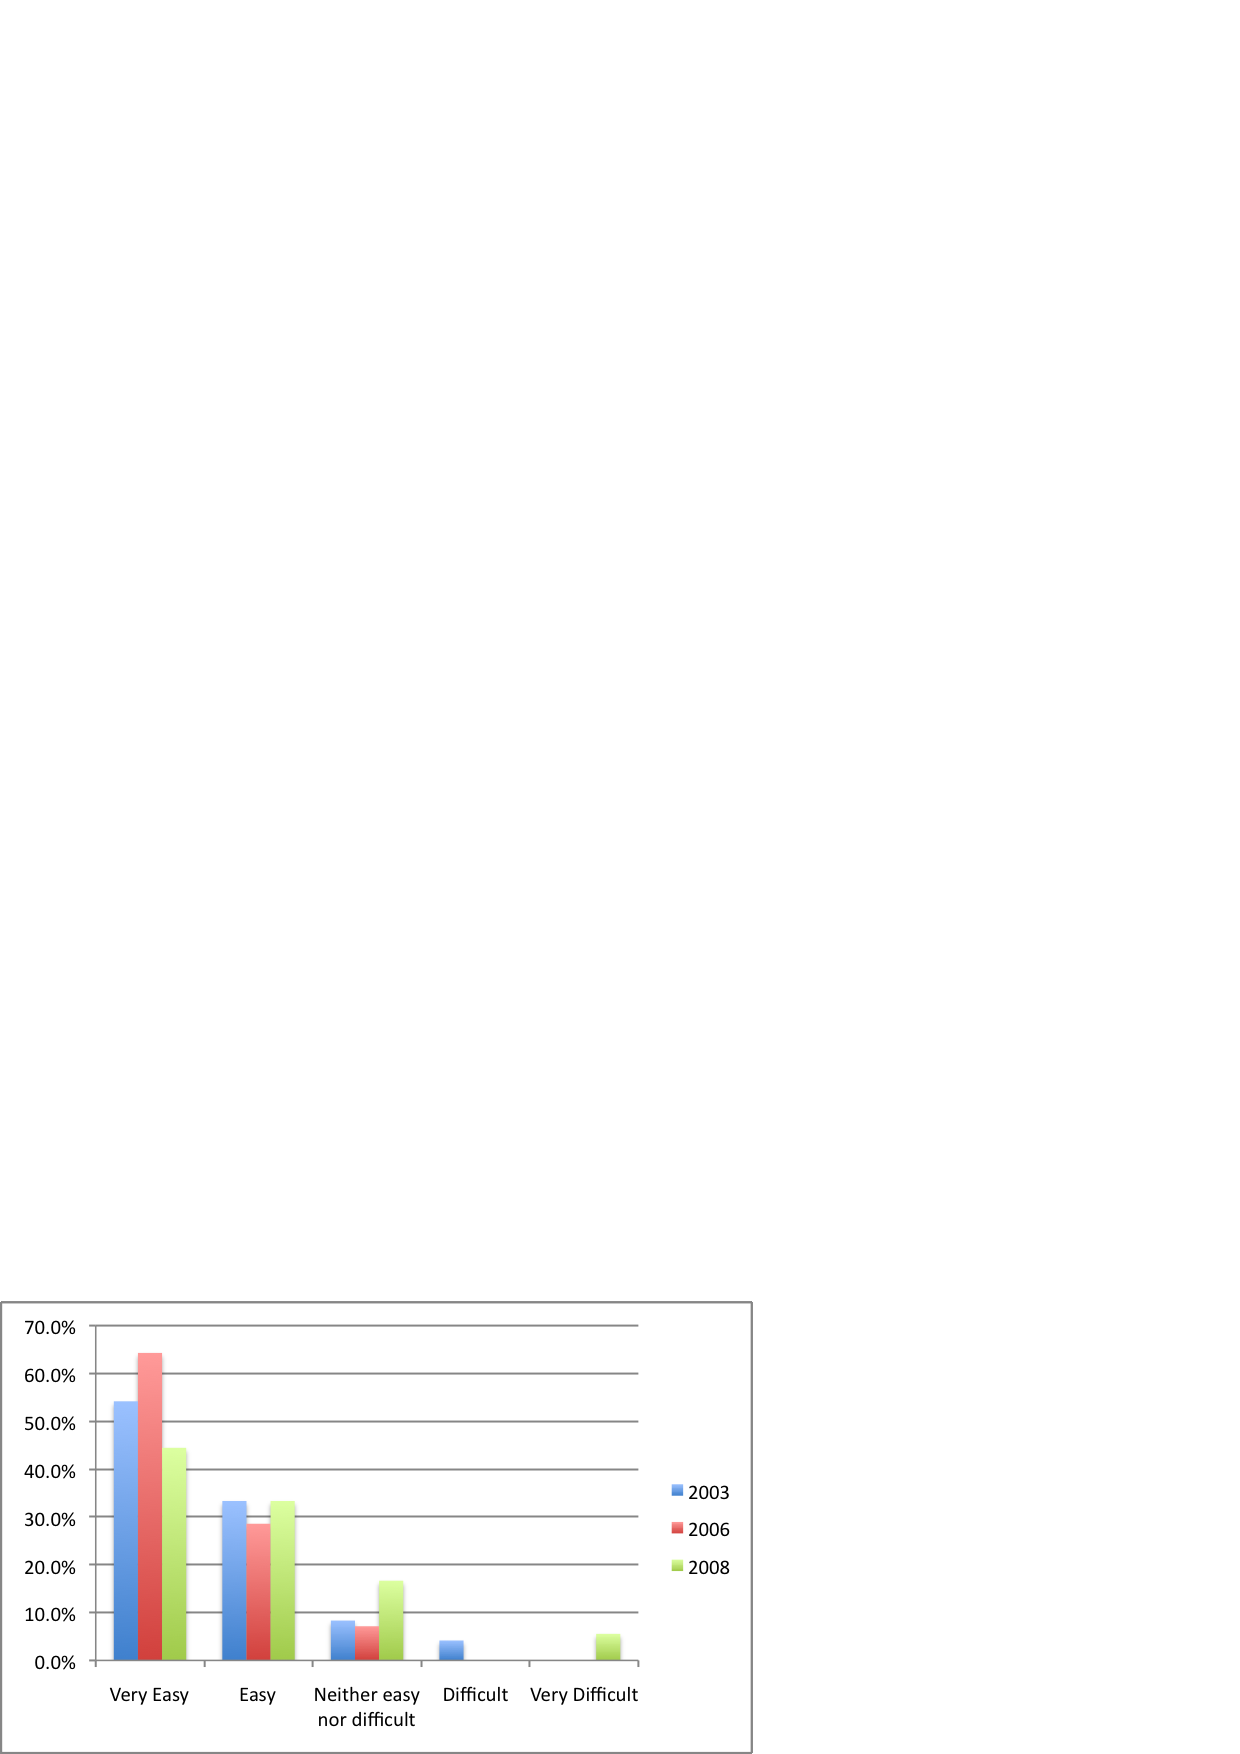
\includegraphics[width=0.6\textwidth]{compare-1} \\ \hline

2. Installing the Ant sensors (JUnit, SCLC, Emma, etc.) was:
\begin{itemize}
\item Very Easy
\item Easy
\item Neither easy nor difficult
\item Difficult
\item Very Difficult
\end{itemize}
&
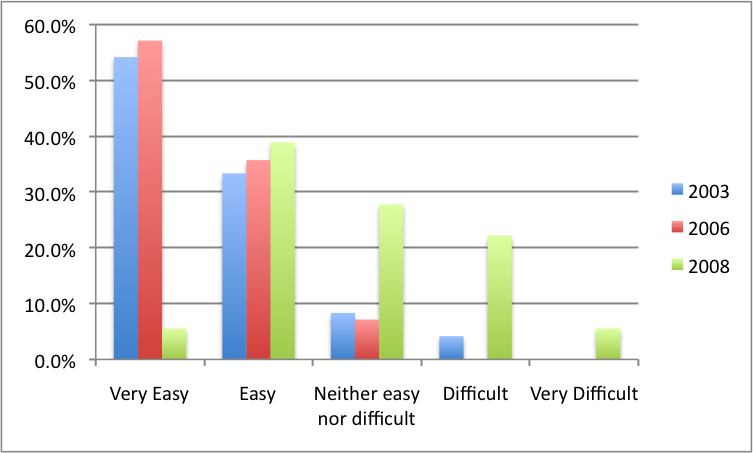
\includegraphics[width=0.6\textwidth]{compare-2} \\ \hline

\end{longtable}
\end{center}

The empirical data indicates that the installation difficulties of both Eclipse sensor and Ant sensors increased in 2008, especially the Ant sensors. Compared to Hackystat in 2006, the major deficiency in installation is the absence of the installer. The distributed documentation instead of a single user manual is another contributor. The setup of SVN sensor and daily build task that collects productive data involves the configuration of Hudson and thus further increase the installation/configuration difficulty.

\subsubsection {Overhead of Use}

\begin{center}
\footnotesize
\begin{longtable}{|m{0.4\textwidth}|m{0.6\textwidth}|}
\hline 
{\bf Question}&{\bf Response}\endhead \hline
4. The amount of overhead required to collect Hackystat data (after successful installation and configuration of sensors) was: *
\begin{itemize}
\item Very Low
\item Low
\item Neither low nor high
\item High
\item Very High
\end{itemize}
&
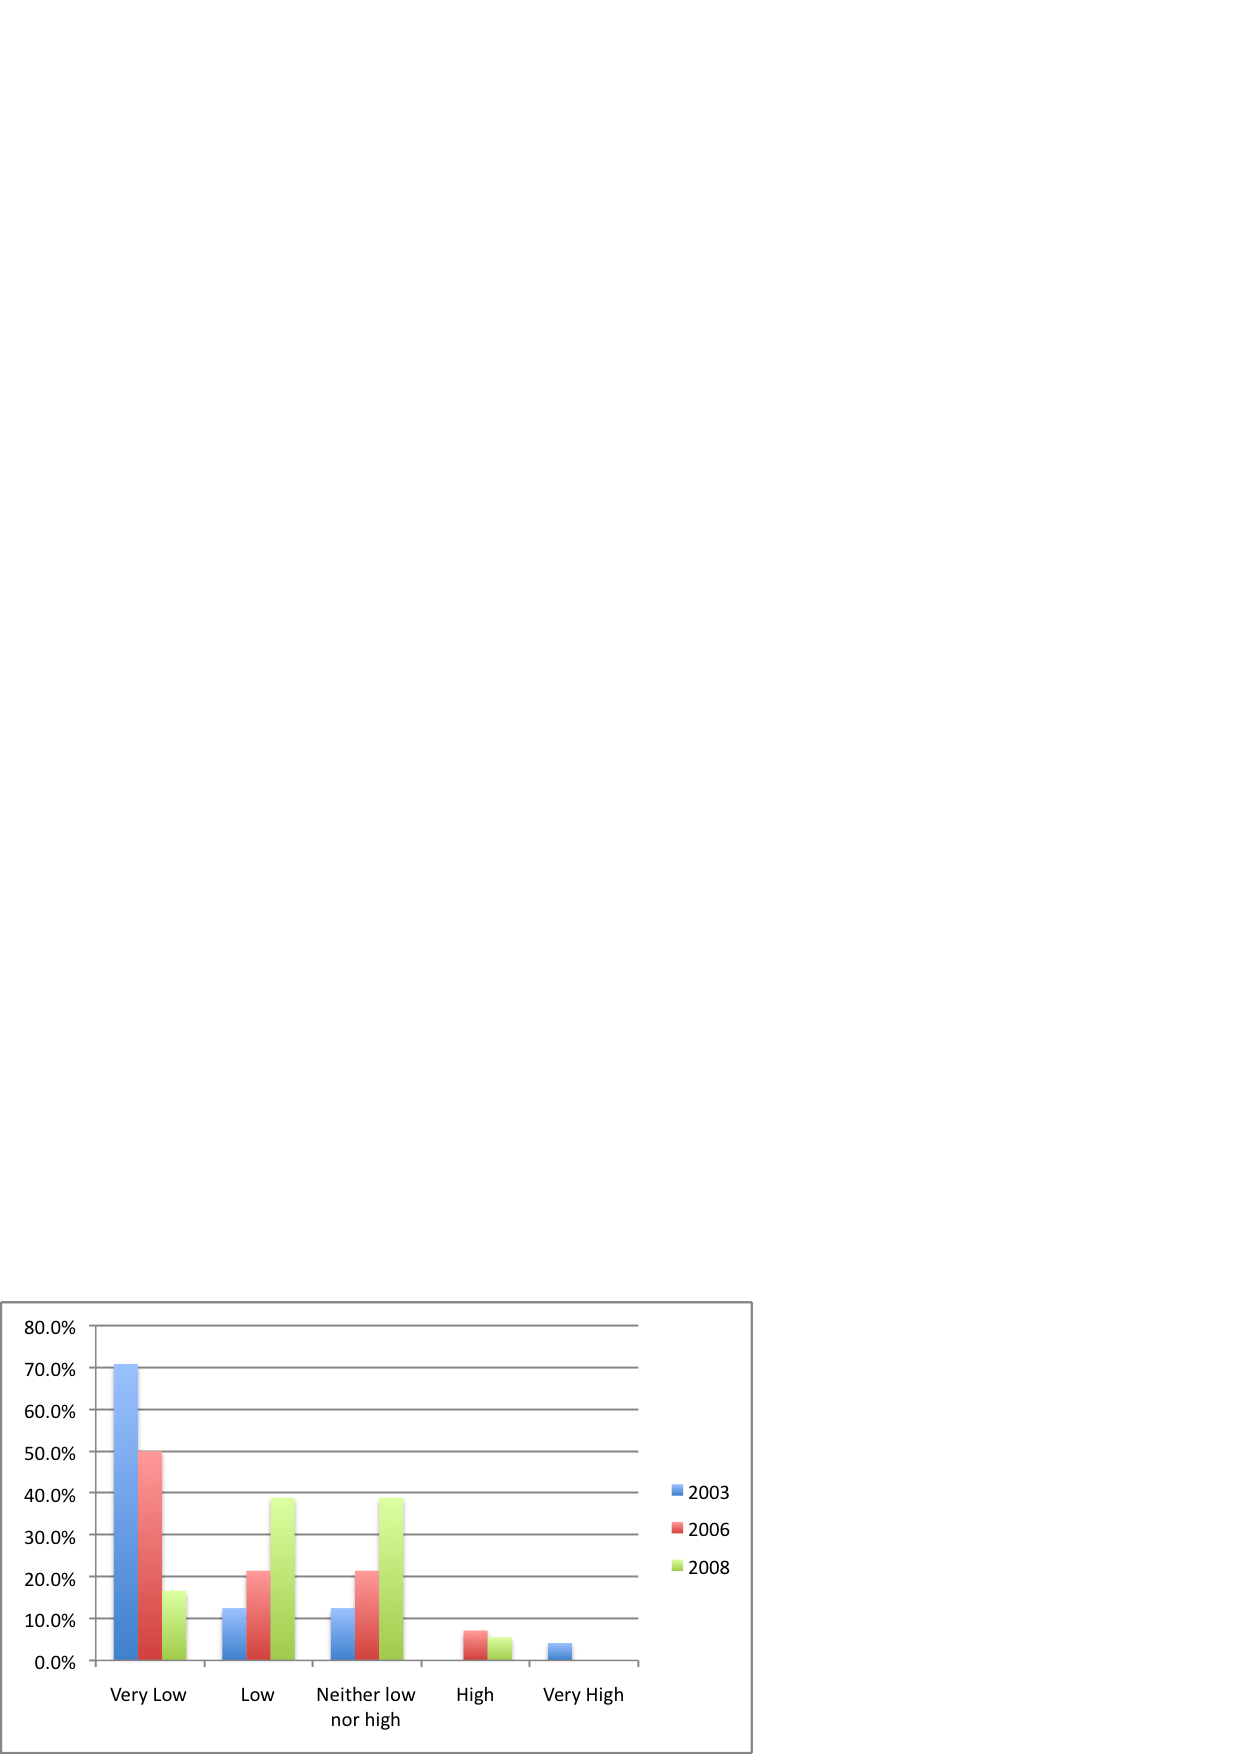
\includegraphics[width=0.6\textwidth]{compare-4} \\ \hline

5. The amount of overhead required to run Hackystat analyses was: *
\begin{itemize}
\item Very Low
\item Low
\item Neither low nor high
\item High
\item Very High
\end{itemize}
&
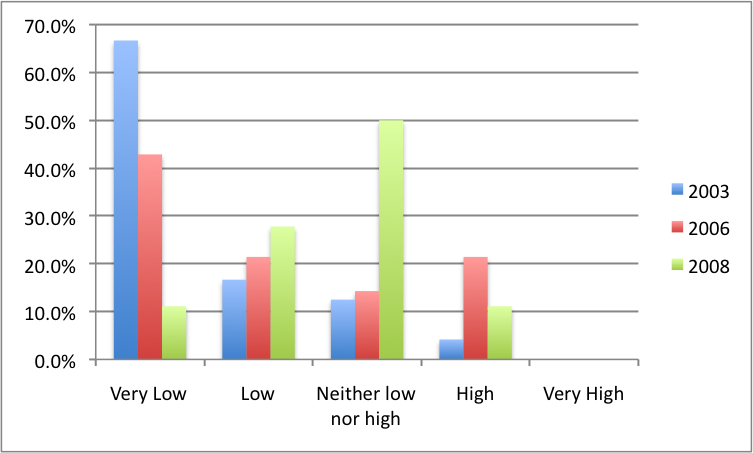
\includegraphics[width=0.6\textwidth]{compare-5} \\ \hline

\end{longtable}
\end{center}
It is surprise that the overhead of use is considered to be higher in 2008. However, the major contributor is different. 

In 2003 and 2006, Ant tasks had to be executed manually everyday in order to ensure no days without data, and it was the major contributor to the overhead of collecting data. In 2008, no daily manual work is required, daily sensor data is collected by the auto daily build in Hudson. However, students complained that the execution time of Ant builds are too long and they considered this to be the major overhead of collecting data. But in fact, running Ant builds were not required by collecting sensor data. Instead, it is a part of the practice of agile development in order to verify the correctness of the code before committing to repository. It was introduced to them along with Hackystat, and this might be the reason that students got confused. 

After the overhead of running Hackystat analyses increased slightly in 2006, it further increased in 2008. But there is no feedback about what factor lead to this high overhead. One of the major factors might be the processing time of SICU analysis, which usually took several minutes to finish. 


\subsubsection {Future Feasibility}

\begin{center}
\footnotesize
\begin{tabular}{|m{0.4\textwidth}|m{0.6\textwidth}|}
\hline 
{\bf Question} & {\bf Response} \\ \hline
16. If I was a professional software developer, using Hackystat at my job would be: *
\begin{itemize}
\item Very feasible
\item Somewhat feasible
\item Neither feasible nor infeasible
\item Somewhat infeasible
\item Very infeasible
\end{itemize}
&
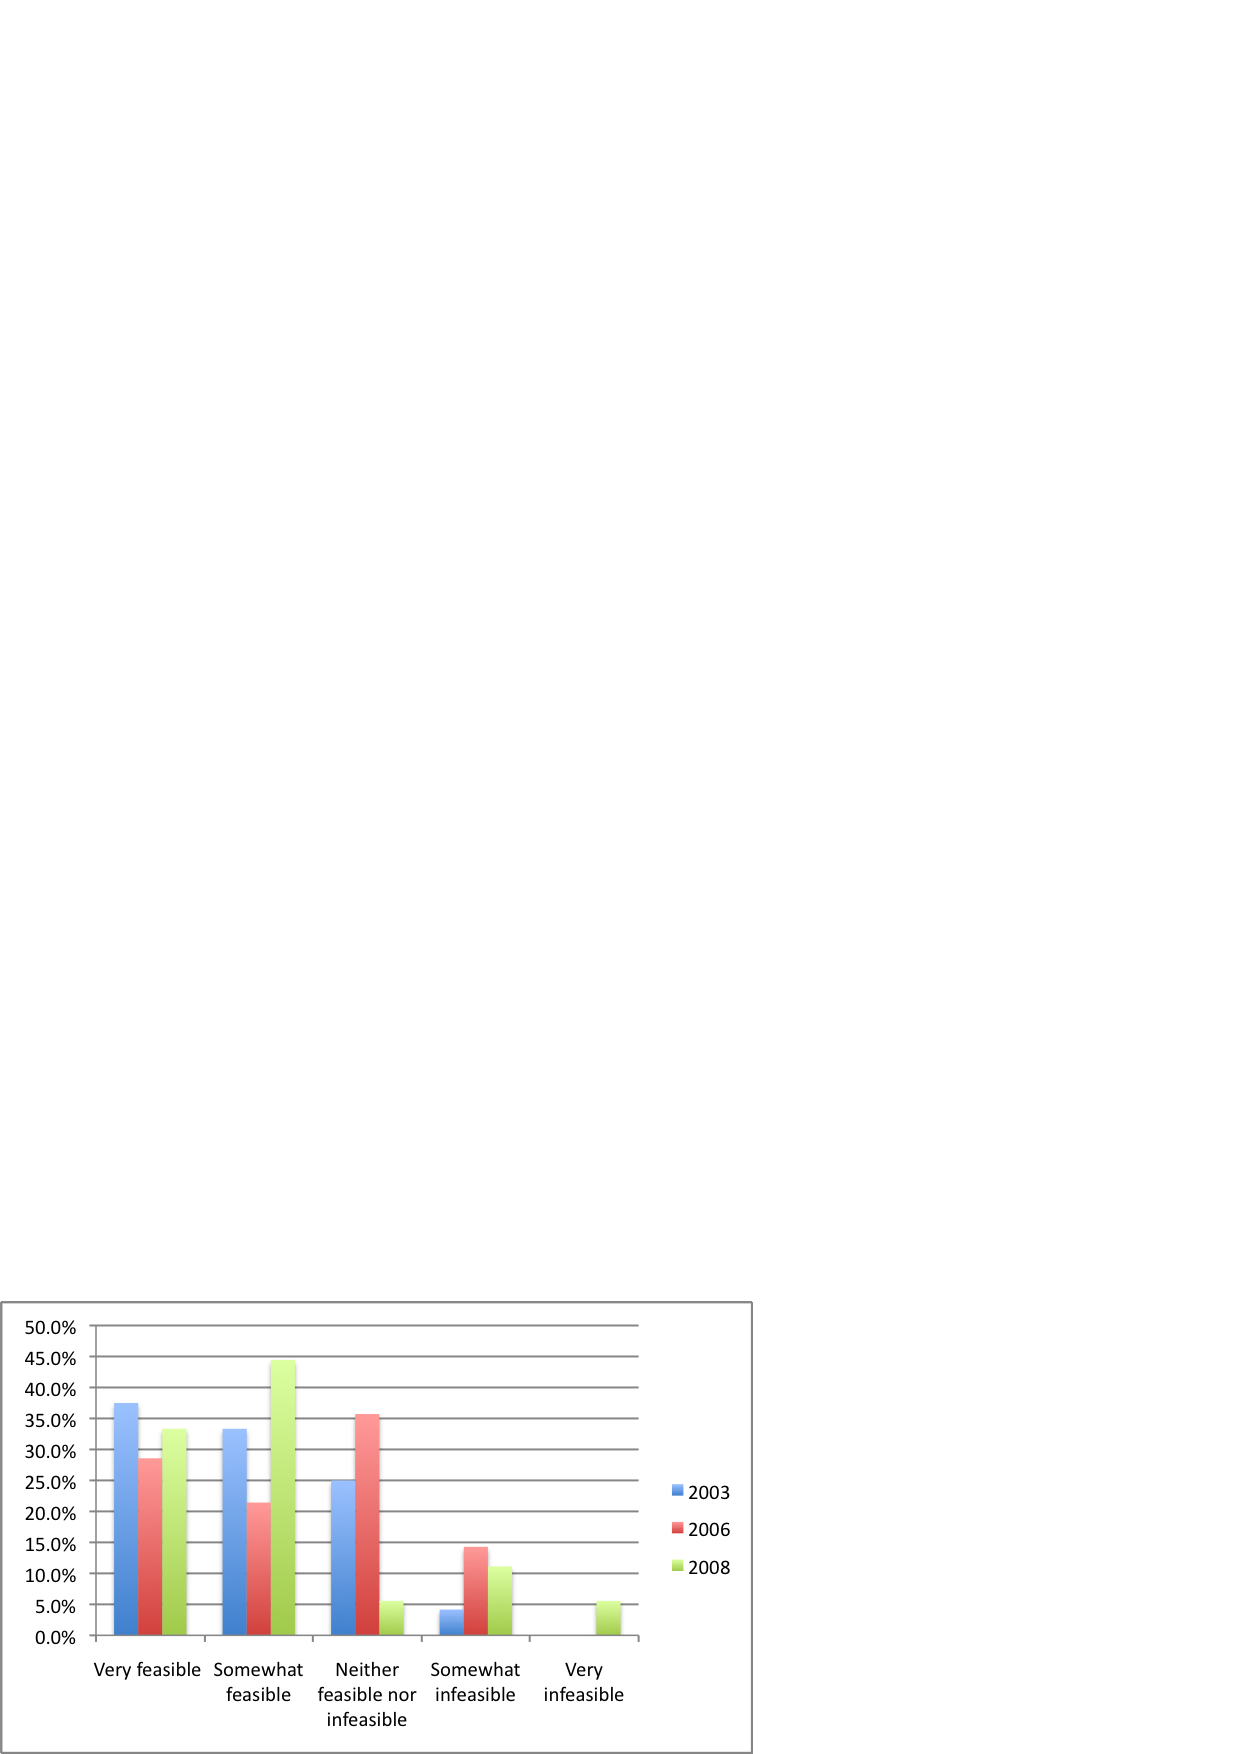
\includegraphics[width=0.6\textwidth]{compare-16} \\ \hline

\end{tabular}
\end{center}

The data indicates that student feelings toward ``professional feasibility'' increased since 2006 and was the highest among the three evaluations. It is an interesting finding because both installation/configuration difficulties and overhead of use increased since 2006. This might be a reflection of increase in utility.

\section{Future Directions}
As the previous section indicates, installation and performance are the major factors that stop users from adopting Hackystat to their daily development. The data accuracy and representation are also need to improve. The following sections will describe some ideas of further enhancement.

\subsection{Installer} 
The installation difficulty is the primary barrier for new users to Hackystat. It should not be too difficult to implement one, especially it was implemented before. Hackystat will gain much free credits from a installer because it will boost the increase in user population and make it less Hackystat-expert only. For users that are not familiar with writing Ant tasks, the installer should also provide a set of templates of Ant build tasks that collect sensor data.

\subsection{Performance of Ant Build Tasks} 
Though there is nothing we can do to improve the performance of the tools used in Ant builds, there is an improvement we can make. That is to reduce the execution times of unit tests to one in verification build. Currently the verification.build.xml, which is commonly used as template for new projects, executes the unit tests twice, one for JUnit sensor data and the other for EMMA sensor data. While the unit tests cosume most of the execution time of the verification build, it is a great waste of time. And it is possible to achieve.

\subsection{Performance of Analysis} 
Beside the algorithms to generate the analyses, the REST API is the major cost in processing. It is based on HTTP communication, which is expensive with small piece of data. Thus to reduce the HTTP calls(same as reduce the REST API calls) or , even better, to replace it with direct memory communication in possible environment will be a solution. But we will surely not eliminate the REST API because its the principal contributor to Hackystat's flexibility.

\subsection{Data Accuracy} 
The DevTime is among the most popular metrics. However, it is far from accurate to measure a developer's effort. However, there are too many tools a developer can use to build sensor for each of them. Futhermore, some developing effort is not even made with a computer, such as reading papers. One way to compensate the automatic sensors is to provide a self-report tool for developers to report their effort manually. Though users can cheat on their reports, so can they on a data sensor.

The Coupling is now too sensitive to introduction of new package, thus does not effetively show the structural complexity of the system.

\subsection{Data Presentation in SICU}
There are many place that data presenation can be improved. They include, but are not restricted to following ideas.

First, for better present Coupling data, it should provide a coloring method that classify values within a smaller range to be
good, values within a bigger range to be average, and values out of range to be bad. The trend will be preferred to be stable. Vibrate within average range will be average, and vibrate out of average range will be bad.

Second, not to classify the values of some metrics. Metrics such as complexity and coupling, the preferrence is know to be lower, but good or bad of a certain is not clear. In this case, the value is better not colored, otherwise it will cause confusion or suspection of the metric.

Third, SICU can provide an overall health rating of each project, based on their metrics. It will be a fussy rating like five stars, and user will be able to choose correspondent metrics and their weights. It will be more useful when the number of projects become bigger.

\bibliography{csdl-trs}
\bibliographystyle{plain}

\end{document}
